% \documentclass[journal]{article}

% \usepackage[backend=biber,style=numeric]{biblatex}
% \addbibresource{references.bib}
% \bibliography{references.bib}
% \usepackage{amsmath}
% \usepackage{graphicx}
% \usepackage{subfiles} % <--- This enables modular files
% \usepackage{caption}
% \usepackage{float}


\documentclass[6pt]{article}
\usepackage[margin=1.0in]{geometry}
\usepackage{setspace}
\usepackage[toc,page]{appendix}
\usepackage{amsmath}
\usepackage[none]{hyphenat} % turn hyphenation off by default
\usepackage{graphicx}
\usepackage[toc,page]{appendix}

% \usepackage{tabularx}


\title{COM3001 Assignment}
\author{Aryan Golbaghi \\
Department of Computer Science, University of Sheffield \\
Sheffield, England \\
\texttt{agolbaghi1@sheffield.ac.uk}}

\markboth{Aryan Golbaghi}{COM3001 Assignment}

\begin{document}


\section{Question 1: Dynamical systems}



\subsection{Exercise 1: Lorenz dynamical system}

The Lorenz system is a set of three coupled, nonlinear differential equations \cite{1963JAtS...20..130L},
 which was introduced by Edward Lorenz in 1963 as a simplified model for atmospheric convection.
  Originally it was derived to study weather prediction and its formula can be found at appendix \ref{eq:lorenz}:

It revealed that even deterministic systems can exhibit unpredictable and chaotic behavior. Lorenz's discovery of the sensitive dependence on initial conditions is now known as the "butterfly effect" \cite{apsLorenz2003}: a concept that demonstrates how small changes in the initial state of a system can lead to drastically divergent trajectories over time, and it has transformed the understanding of dynamical systems by showing that small differences in starting states can lead to dramatically divergent results over time.

Historically, the Lorenz system marked a paradigm shift. Before Lorenz's work, many scientists assumed that small changes in initial conditions would only lead to small variations in future behavior. However, Lorenz showed that the weather, which was considered a definitive example of predictable physical systems, could be inherently unpredictable. This insight laid the foundation for modern chaos theory and encouraged extensive research into nonlinear dynamics \cite{apsLorenz2003}.

Beyond its initial role in meteorology, the Lorenz system has found widespread application in various fields. Its conceptual framework has influenced research in fluid dynamics, laser physics, electrical circuits, and even models of population dynamics \cite{kashyap2024lorenz}. In many of these areas, the Lorenz equations serve as a benchmark for studying chaotic attractors, strange attractors, and fractal dimensions, concepts that have proven essential in describing complex and real-world phenomena. The model’s ability to capture the essence of chaotic behavior makes it invaluable not only as a theoretical tool but also as a practical one for understanding and predicting complex systems.

In recent years, the relevance of the Lorenz system has grown further with advances in computational methods and interdisciplinary applications. For instance, researchers have employed data assimilation techniques and machine learning approaches such as reservoir computing to both forecast and analyze chaotic dynamics using the Lorenz attractor as a prototype. These modern developments underscore the system’s enduring importance: they not only provide new tools for dealing with uncertainties in weather forecasting but also offer insights into controlling chaotic systems in engineering and natural sciences \cite{Pathak_2017}. Furthermore, studies exploring quantum computing approaches to analyze the non-Hermitian Jacobian matrix of the Lorenz system have opened promising avenues for future research in atmospheric physics and beyond \cite{armaos2024quantumcomputingatmosphericdynamics}.

Overall, the Lorenz system remains very important in the study of nonlinear dynamical systems. Its historical impact has been reshaping our understanding of predictability and determinism, and it continues to influence modern scientific research. As contemporary studies extend its applications into new fields, the Lorenz model exemplifies how a deceptively simple set of equations can encapsulate the profound behavior of nature, making it directly relevant to a wide array of exercises and research endeavors in mathematical modeling.

\subsubsection{How to use numerical methods to simulate the system, }
As shown in the Lorenz Equation \ref{eq:lorenz}, Because of the system's nonlinearity and sensitivity to initial conditions (the "butterfly effect"), an analytical solution is not feasible. Instead, we can use numerical integration. In this section, I present two methods, alongside an analysis of time step effects and the simulation results:


\subsubsection{The Explicit Euler Method}

The Euler method is a first order numerical scheme. For a general differential equation, the formula can be found in the appendix \ref{eq:euler_lorenz}.

Although this formula is straightforward, the Euler method is only first order accurate; and its error is proportional to $\Delta t$. For the Lorenz system \ref{eq:lorenz}, this may lead to significant inaccuracies when using larger time steps, especially due to the chaotic nature of the system.

\subsubsection{The Fourth-Order Runge-Kutta (RK4) Method}

RK4 is a more accurate method that uses intermediate calculations to achieve fourth-order accuracy. The RK4 update rule for the Lorenz system is given by the formula in the appendix \ref{eq:rk4_lorenz}. This method is more computationally intensive than Euler's method, but it provides a much better approximation of the true solution, especially for larger time steps.
The RK4 method is particularly effective for systems like the Lorenz equations, where the dynamics can change rapidly. By using multiple intermediate steps to calculate the slope, RK4 captures the curvature of the solution trajectory more accurately than Euler's method, which only uses the slope at the beginning of the interval. This results in a more stable and accurate approximation of the system's behavior over time.
The RK4 method is widely used in various fields, including physics, engineering, and finance, where accurate numerical solutions to differential equations are required. Its ability to handle stiff equations and chaotic systems makes it a valuable tool for researchers and practitioners alike.

\subsubsection{Time Step Analysis}

Choosing an appropriate $\Delta t$ is crucial:

\begin{itemize}
    \item \textbf{Smaller} $\Delta t$ (e.g., 0.01, 0.001) improves accuracy by capturing more details of the system’s dynamics but increases computation expenses.
    \item \textbf{Larger} $\Delta t$ (e.g., 0.05, 0.08) may be computationally cheaper but can lead to numerical instability and incorrect behavior in the simulation.
\end{itemize}
While fixed time step methods such as Euler and RK4 are usefull, adaptive integration methods like Runge-Kutta-Fehlberg (RK45) can automatically adjust $\Delta t$ based on local error estimates. This adaptive control is particularly useful in chaotic systems, where the dynamics can vary significantly over time, ensuring both efficiency and robustness in long-term simulations. By dynamically allocating computational resources, reducing the step size in regions of rapid change and increasing it in smoother regions, adaptive methods not only maintain accuracy but also improve performance.


\subsubsection{Simulation and Results}
The simulations were conducted using both the Explicit Euler and the Fourth-Order Runge-Kutta (RK4) methods over a total simulation time of 40 seconds \cite{youngaryanLorenzPlot1.1.4}. Several time step sizes were considered, ranging from small steps ($\Delta t = 0.001$) up to larger steps ($\Delta t = 0.1$). The results of the simulations are presented in the following figures \ref{fig:lorenz_vis}, \ref{fig:error_comparison1.1.4}:


My observations for different time steps are as follows:
\textbf{Small} $\Delta t$ (e.g., 0.001): Both methods yield a stable, accurate Lorenz attractor. RK4 shows less numerical distortion than Euler.\\

\textbf{Intermediate} $\Delta t$ (0.01): Euler solutions begin to show noticeable distortion. RK4 typically remains close to the true attractor, but still accumulates some error.\\

\textbf{Large} $\Delta t$ (0.1): Euler diverges dramatically. RK4 diverges from the solution too, however the RK4 method stays more loyal to the true solution.

In figure \ref{fig:error_comparison1.1.4} shows that the Euler method is conditionally stable, meaning that for chaotic systems like the Lorenz system, even small time steps might lead to instability over long simulations, however the RK4 method has a larger stability region, which is why it can both stay stable and performs better at larger time steps compared to Euler.

\subsubsection{Quantitative Error Analysis}

To assess the performance of the numerical methods, we compare the computed trajectories to a high-accuracy reference solution obtained with the RK4 method at a very small time step (\(\Delta t = 0.001\)). In this context, the accuracy of a method is quantified by the \emph{average Euclidean error}, as defined in the appendix \ref{eq:error_metric}.


\paragraph{Theoretical Error Scaling:}
It is well known that different numerical integration methods exhibit distinct error behaviors:

\begin{itemize}
    \item \textbf{Euler Method:} The Euler method has a \emph{local truncation error} on the order of \(O(\Delta t^2)\). However, because errors accumulate over \(T/\Delta t\) steps, the \emph{global error} scales as \(O(\Delta t)\) (i.e., linearly with the time step). This implies that even small increases in \(\Delta t\) will lead to a proportional increase in the total error.
    \item \textbf{Fourth-Order Runge-Kutta (RK4) Method:} In contrast, the RK4 method exhibits a much smaller local truncation error of \(O(\Delta t^5)\), resulting in a global error that scales as \(O(\Delta t^4)\). This steep reduction in error with decreasing \(\Delta t\) makes RK4 far more accurate for the same step sizes.
\end{itemize}

The simulation results align with these theoretical expectations. For example, as seen in Figure~\ref{fig:lorenz_error}, when the time step increases beyond \(0.01\), the Euler method's error grows rapidly, failing to accurately reproduce the Lorenz attractor. In contrast, the RK4 method maintains a significantly lower error, demonstrating its superior stability and accuracy even at moderately larger time steps.

\paragraph{Error Metric Details:}
The average Euclidean error is computed by comparing the solution at each time step from the numerical method under investigation with the corresponding state of the reference solution. By averaging the Euclidean distances over all time steps, we obtain a single scalar measure of the overall deviation. This metric provides a straightforward yet effective means to quantify how numerical errors accumulate over time, particularly in chaotic systems where small errors can lead to substantial deviations in the trajectory.

Overall, these analyses not only confirm the expected theoretical error scaling for each method but also emphasize the critical importance of choosing appropriate time steps when simulating sensitive, nonlinear systems such as the Lorenz attractor.

% \subfile{../figures/fig.tex}

\section{Exercise 2: Selecting a Numerical Method and Demonstrating Chaotic Behavior}

\subsubsection{Selection of Numerical Method and Time Step}
Based on the analyses in Exercises 1.2.4 and 1.2.5, I have chosen the Fourth-Order Runge-Kutta (RK4) method for simulating the Lorenz system.
The choice of the RK4 method is supported by the following considerations:

\begin{itemize}
    \item \textbf{Accuracy:} As illustrated in Figure \ref{fig:error_comparison_same_times} and Table \ref{tab:integration_methods}, the RK4 method exhibits substantially lower local truncation errors compared to the Euler method, making it more reliable in capturing the intricate dynamics of the system.
    \item \textbf{Stability:} Experimental results (see Figure \ref{fig:lorenz_error1000}) indicate that the Euler method becomes unstable for time steps exceeding \(\Delta t > 0.025\). In contrast, RK4 remains stable even for time steps as large as \(\Delta t = 0.13\) (see \ref{fig:error_comparison_rk4_stable_0.13}), proving its robustness for simulating chaotic systems.
    \item \textbf{Computational Efficiency:} Although smaller time steps can improve accuracy, they also lead to higher computational costs. To strike an appropriate balance between accuracy and efficiency, I employed a hyperparameter optimization approach using the Optuna library \cite{akiba2019optuna} (see also my implementation in \cite{youngaryanOptunaCode}). A sensitivity analysis was conducted by varying \(\Delta t\) using the objective function (\ref{eq:composite_objective}). This analysis confirmed that a time step of \(\Delta t = 0.0073\) (see Figure \ref{fig:optuna_lorenz_3d} for comparison).
\end{itemize}

\noindent
Optimization was guided by a \textbf{composite objective function}, which incorporates both the simulation error and a proxy for computational cost:

% \begin{equation}
% \text{Error} = \frac{1}{N} \sum_{i=1}^{N} \left\| \mathbf{x}_{\text{sim}}(t_i) - \mathbf{x}_{\text{ref}}(t_i) \right\|_2
% \label{eq:mean_euclidean_error}
% \end{equation}
\begin{equation}
\text{Composite Objective} = \frac{1}{N} \sum_{i=1}^{N} \left\| \mathbf{x}_{\text{sim}}(t_i) - \mathbf{x}_{\text{ref}}(t_i) \right\|_2 + \alpha \cdot \left( \frac{T}{\Delta t} \right)
\label{eq:composite_objective}
\end{equation}

\begin{align*}
\text{where:} \quad
& \mathbf{x}_{\text{sim}}(t_i) \text{ is the simulated state at time } t_i, \\
& \mathbf{x}_{\text{ref}}(t_i) \text{ is the reference state at time } t_i, \\
& N \text{ is the number of time steps in the simulation}, \\
& \left\| \cdot \right\|_2 \text{ denotes the Euclidean (L2) norm}, \\
& \alpha \text{ is a weighting factor for the cost term, with } \alpha = 0.0009 \text{ in this case}, \\
& T \text{ is the total simulation time}, \\
& \Delta t \text{ is the time step used.}
\end{align*}

\noindent
This formulation encourages the optimizer to select a time step that balances simulation accuracy with computational efficiency, avoiding excessively fine resolutions. However, its performance may depend on the specific weighting parameter $\alpha$ (manually tuned here) and the reference system used.


\subsubsection{Generation and Analysis of Phase Portraits}
To demonstrate the characteristic chaotic behavior ("butterfly effect") of the Lorenz system, I have chosen two similar initial conditions of (0.01, 2.0, 1.0) and (0.1, 2.0, 1.0) and the time steps of \(\Delta t = 0.0073\).

Figures \ref{fig:two_initial_conditions_3d_separate}, \ref{fig:two_initial_conditions_3d_separate_2} and \ref{fig:two_initial_conditions_3d_separate_3} display these phase portraits. Although the initial conditions differ only in the $x$ component by a small amount, the resulting trajectories clearly exhibit chaotic divergence over time, Both portraits exhibit the same broad “butterfly” structure, but their trajectories do not remain synchronized. As time goes on, the small difference amplifies until the solutions appear uncorrelated.

\subsection{What Does It Mean for a System to Be Chaotic?}
A chaotic system is a deterministic system that is unpredictable and seemingly random behavior due to its extreme sensitivity to initial conditions. This means that even very small differences in starting conditions can lead to completely different outcomes over time. Such systems are characterized by aperiodic long-term behavior, meaning they do not settle into regular cycles, and their evolution over time appears disorderly despite being governed by deterministic laws.

for more details on variances in in the initial condition more details can be found in theb \textbf{Generation and Analysis of Phase Portraits} section.
\section{Question 2: Prey-Predator System}
\section{Simulate the prey-predator model}

The result of the prey-predator simulation can be found at Figures (\ref{fig:Ecolab_pred_prey}, \ref{fig:Ecolab_pred_prey_no_foxes}), here is a description of the simulation:

In the simulation, we can see an oscillatory behavior of the populations, which is a characteristic feature of predator-prey dynamics.
\begin{itemize}
    \item Grass (black curve) grows, fueling an increase in Rabbits (orange).
    \item As rabbits grow numbers, Foxes (blue) find abundant prey, so fox numbers grow.
    \item Increasing the number of rabbits will cause to decrease the amount of grass (this is seen in Figure \ref{fig:Ecolab_pred_prey_no_foxes} too).
    \item Once foxes grow in numbers and the grass amount decreases because of the population of rabbits, the population of rabbits will decrease.
    \item As the number of rabbits decreases, the foxes will have less food, leading to a decrease in their population.
    \item as there is less rabbits, the grass will grow again, and the cycle will repeat.
\end{itemize}

The intreating findings I can see from this simulation is even though the agent based model includes randomized movement and local interactions, the overall population still exhibits an oscillatory up and down cycles, similar to what we see in standard predator prey models (Lotka Volterra curves which mentioned in the lectures).


\section{Differences between Agent Based Modeling vs Equation Based Modeling}

In a classical equation based (ODE) predator prey model, such as Lotka Volterra equations:
\[
\left\{
\begin{aligned}
\frac{dx}{dt} &= x(\alpha - \beta y) \\
\frac{dy}{dt} &= y(\delta x - \gamma)
\end{aligned}
\right.
\qquad
\begin{aligned}
\alpha &> 0, \quad \text{Reproduction prey} \\
\beta &> 0, \quad \text{Predation} \\
\gamma &> 0, \quad \text{Extinction predator} \\
\delta &> 0, \quad \text{Reproduction predator}
\end{aligned}
\]

populations are treated as continuous, homogeneous averages. By contrast, agent based models (ABMs) track individual rabbits and foxes.
I have summarized the key differences between these two models in the following (see this table \ref{tab:diff_two_models_predator_prey}):

\begin{itemize}
    \item \textbf{Spatial Heterogeneity}
    \begin{itemize}
        \item \textbf{ABM:} Rabbits and foxes move around, so local depletion of grass or clustering of rabbits affects local outcomes. Some regions can be overgrazed or overhunted while others remain safe havens, and these local effects alter the overall population dynamics.
        \item \textbf{ODE:} Assumes well mixed populations with no spatial structure. Grass, rabbits, and foxes interact uniformly in a single compartment.
    \end{itemize}
    
    \item \textbf{Discrete and Stochastic Interactions}
    \begin{itemize}
        \item \textbf{ABM:} Each eating or breeding event is discrete. Foxes may or may not successfully catch a rabbit (random probability), and rabbits may or may not find enough grass. This random element leads to fluctuations around the average trend.
        \item \textbf{ODE:} Uses deterministic rate equations; there is no randomness in who gets eaten or how far you can move.
    \end{itemize}
    
    \item \textbf{Individual Traits and Thresholds}
    \begin{itemize}
        \item \textbf{ABM:} Each agent has individual properties such as an internal food store, an age, and breeding frequency. Once a rabbit's internal food is depleted, it dies—even if the average rabbit might have enough food.
        \item \textbf{ODE:} Tracks the average rate of consumption and reproduction. There is no notion of an individual's internal energy or local shortage.
    \end{itemize}
    
    \item \textbf{Emergent Behavior and Local Extinction}
    \begin{itemize}
        \item \textbf{ABM:} Because movement is localized, pockets of rabbits or foxes can go extinct locally while others flourish elsewhere. Over time, random events can create drastically different patterns across multiple simulations.
        \item \textbf{ODE:} Typically yields a single smooth trajectory for each initial condition—no chance of a local "pocket" dying off on its own.
    \end{itemize}
    
    \item \textbf{Complexity vs. Analytical Tractability}
    \begin{itemize}
        \item \textbf{ABM:} More realistic in capturing how individuals actually move, eat, and breed, but more complex and computationally intensive. Hard to get a neat "closed form" solution.
        \item \textbf{ODE:} Mathematically elegant with known analysis techniques (e.g., stability analysis, limit cycles). Faster to run and simpler to interpret but less nuanced spatially and individually.
    \end{itemize}
\end{itemize}

\subsection[short]{Why Do Results Differ Across Runs?}

\begin{itemize}
    \item \textbf{Random Initial Conditions}
    \begin{itemize}
        \item Each run places rabbits and foxes at random locations in the grid.
        \item Grass regeneration also occurs in randomly chosen cells.
    \end{itemize}

    \item \textbf{Probabilistic Movement and Interactions}
    \begin{itemize}
        \item Rabbits choose random directions if no grass is found in sight.
        \item Foxes move randomly and only sometimes succeed in catching a rabbit (based on a probability that depends on the distance).
        \item Each new rabbit or fox gets a random starting age, This affects how soon they die or reproduce.
    \end{itemize}

\end{itemize}

\subsection[short]{Simulating the ABM Model to Monitor the Change of Key Variables}
\section{Parameter Sensitivity Analysis }

In the previous exercise, we observed that the fox population went extinct in 6 out of 100 simulation runs. In this section, I aim to identify the conditions under which the fox population can be sustained more consistently. To do this, I selected a key parameter to vary and recorded the system's behavior in response.

The primary cause of fox extinction appears to be a shortage of rabbits, which in turn is often caused by a lack of grass, the main food source for rabbits. Therefore, I decided to vary the \texttt{growrate} parameter of the environment, which controls how many new grass units are added to the grid in each iteration. By increasing the grow rate, I aim to assess whether more abundant grass leads to larger rabbit populations, and subsequently, to better survival conditions for foxes.







\newpage
\appendix

\section{Mathematical Formulations}

\begin{equation}\label{eq:lorenz}
\frac{dx}{dt} = \sigma(y - x), \quad
\frac{dy}{dt} = x(\rho - z) - y, \quad
\frac{dz}{dt} = xy - \beta z
\end{equation}

\begin{center}
where $\sigma = 10$, $\rho = 28$, and $\beta = \frac{8}{3}$.
\end{center}


\begin{equation}\label{eq:euler_lorenz}
    \begin{aligned}
    \frac{dx}{dt} &= f(x), \\
    x_{n+1} &= x_n + \Delta t\, \sigma (y_n - x_n), \\
    y_{n+1} &= y_n + \Delta t\, [x_n(\rho - z_n) - y_n], \\
    z_{n+1} &= z_n + \Delta t\, [x_n y_n - \beta z_n]
    \end{aligned}
    \end{equation}
    
    \begin{center}
    where $\Delta t$ is the time step.
\end{center}
    
\begin{equation}
    \begin{aligned}
    k_1 &= f(x_n, y_n, z_n), \\
    k_2 &= f\left(x_n + \tfrac{1}{2} \Delta t\, k_{1,x},\; y_n + \tfrac{1}{2} \Delta t\, k_{1,y},\; z_n + \tfrac{1}{2} \Delta t\, k_{1,z} \right), \\
    k_3 &= f\left(x_n + \tfrac{1}{2} \Delta t\, k_{2,x},\; y_n + \tfrac{1}{2} \Delta t\, k_{2,y},\; z_n + \tfrac{1}{2} \Delta t\, k_{2,z} \right), \\
    k_4 &= f\left(x_n + \Delta t\, k_{3,x},\; y_n + \Delta t\, k_{3,y},\; z_n + \Delta t\, k_{3,z} \right), \\
    x_{n+1} &= x_n + \frac{\Delta t}{6} \left( k_{1,x} + 2k_{2,x} + 2k_{3,x} + k_{4,x} \right), \\
    y_{n+1} &= y_n + \frac{\Delta t}{6} \left( k_{1,y} + 2k_{2,y} + 2k_{3,y} + k_{4,y} \right), \\
    z_{n+1} &= z_n + \frac{\Delta t}{6} \left( k_{1,z} + 2k_{2,z} + 2k_{3,z} + k_{4,z} \right)
    \label{eq:rk4_lorenz}
    \end{aligned}
\end{equation}
    

\begin{equation}\label{eq:error_metric}
    \text{Error} = \frac{1}{N} \sum_{i=1}^{N} 
    \bigl\| \mathbf{X}_i^{\text{method}} - \mathbf{X}_i^{\text{ref}} \bigr\|
    \end{equation}
    
    \noindent
    where \(\mathbf{X}_i = (x_i, y_i, z_i)\) represents the state vector at the \(i\)th time step, \(\mathbf{X}_i^{\text{method}}\) is the solution produced by the numerical method being tested, and \(\mathbf{X}_i^{\text{ref}}\) is the corresponding state from the reference trajectory.
    

    \begin{equation}
        \text{Composite Objective} = \frac{1}{N} \sum_{i=1}^{N} \left\| \mathbf{x}_{\text{sim}}(t_i) - \mathbf{x}_{\text{ref}}(t_i) \right\|_2 + \alpha \cdot \left( \frac{T}{\Delta t} \right)
        \label{eq:composite_objective}
        \end{equation}
        
        \begin{align*}
        \text{where:} \quad
        & \mathbf{x}_{\text{sim}}(t_i) \text{ is the simulated state at time } t_i, \\
        & \mathbf{x}_{\text{ref}}(t_i) \text{ is the reference state at time } t_i, \\
        & N \text{ is the number of time steps in the simulation}, \\
        & \left\| \cdot \right\|_2 \text{ denotes the Euclidean (L2) norm}, \\
        & \alpha \text{ is a weighting factor for the cost term, with } \alpha = 0.0009 \text{ in this case}, \\
        & T \text{ is the total simulation time}, \\
        & \Delta t \text{ is the time step used.}
        \end{align*}
        
        \noindent
        This formulation encourages the optimizer to select a time step that balances simulation accuracy with computational efficiency, avoiding excessively fine resolutions. However, its performance may depend on the specific weighting parameter $\alpha$ (manually tuned here) and the reference system used.
        

\begin{equation}\label{eq:predator_prey}
            \left\{
            \begin{aligned}
            \frac{dx}{dt} &= x(\alpha - \beta y) \\
            \frac{dy}{dt} &= y(\delta x - \gamma)
            \end{aligned}
            \right.
            \qquad
            \begin{aligned}
            \alpha &> 0, && \text{(Reproduction of prey)} \\
            \beta &> 0, && \text{(Predation rate)} \\
            \gamma &> 0, && \text{(Extinction of predator)} \\
            \delta &> 0, && \text{(Reproduction of predator)}
            \end{aligned}
\end{equation}
            


\section{images}
\listoffigures
\begin{figure}[!ht]
  \centering
  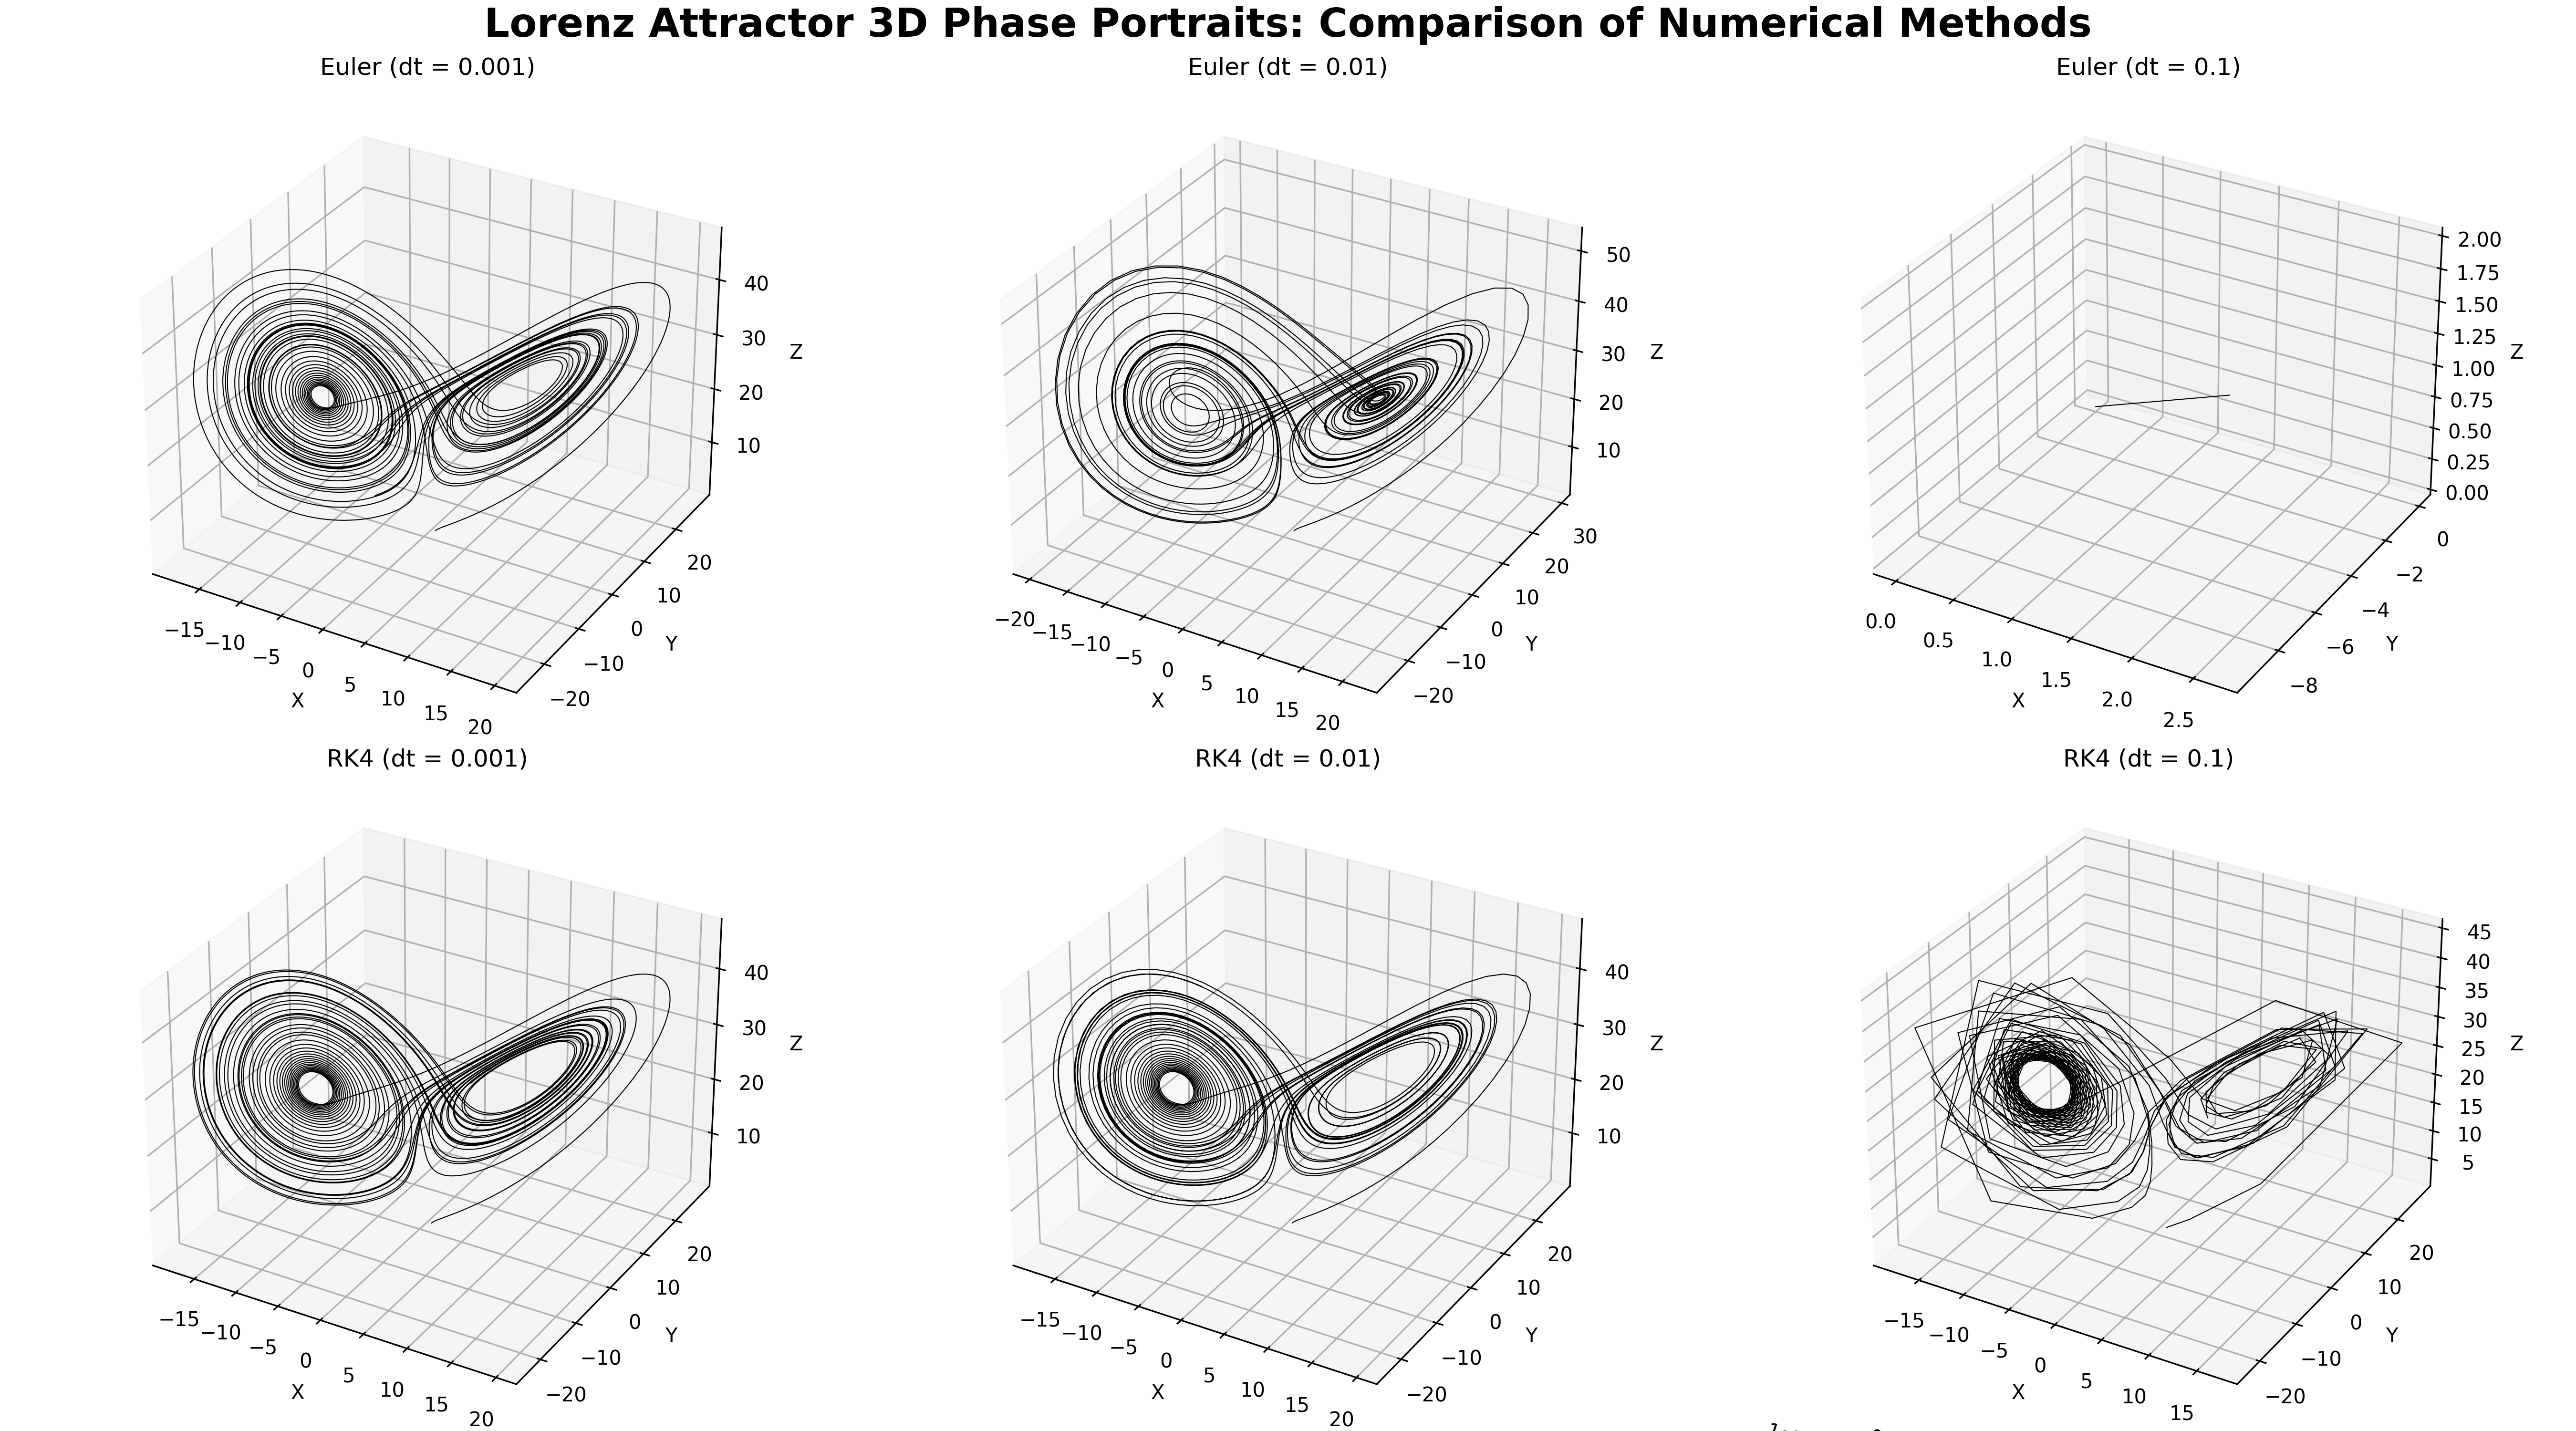
\includegraphics[width=1.0\linewidth]{images/phase_portraits1.1.4.png} 
  \caption{Lorenz attractor with initial state (1.0,1.0,1.0) and time step (0.001, 0.01, 0.1), and total simulation time of 40 seconds,  For $\Delta t > 0.01$, the solution is not stable enough to reliably reproduce the attractor shape\cite{youngaryanLorenzPlot1.1.4_image}}
  \label{fig:lorenz_vis}
\end{figure}


\begin{figure}[!ht]
  \centering
  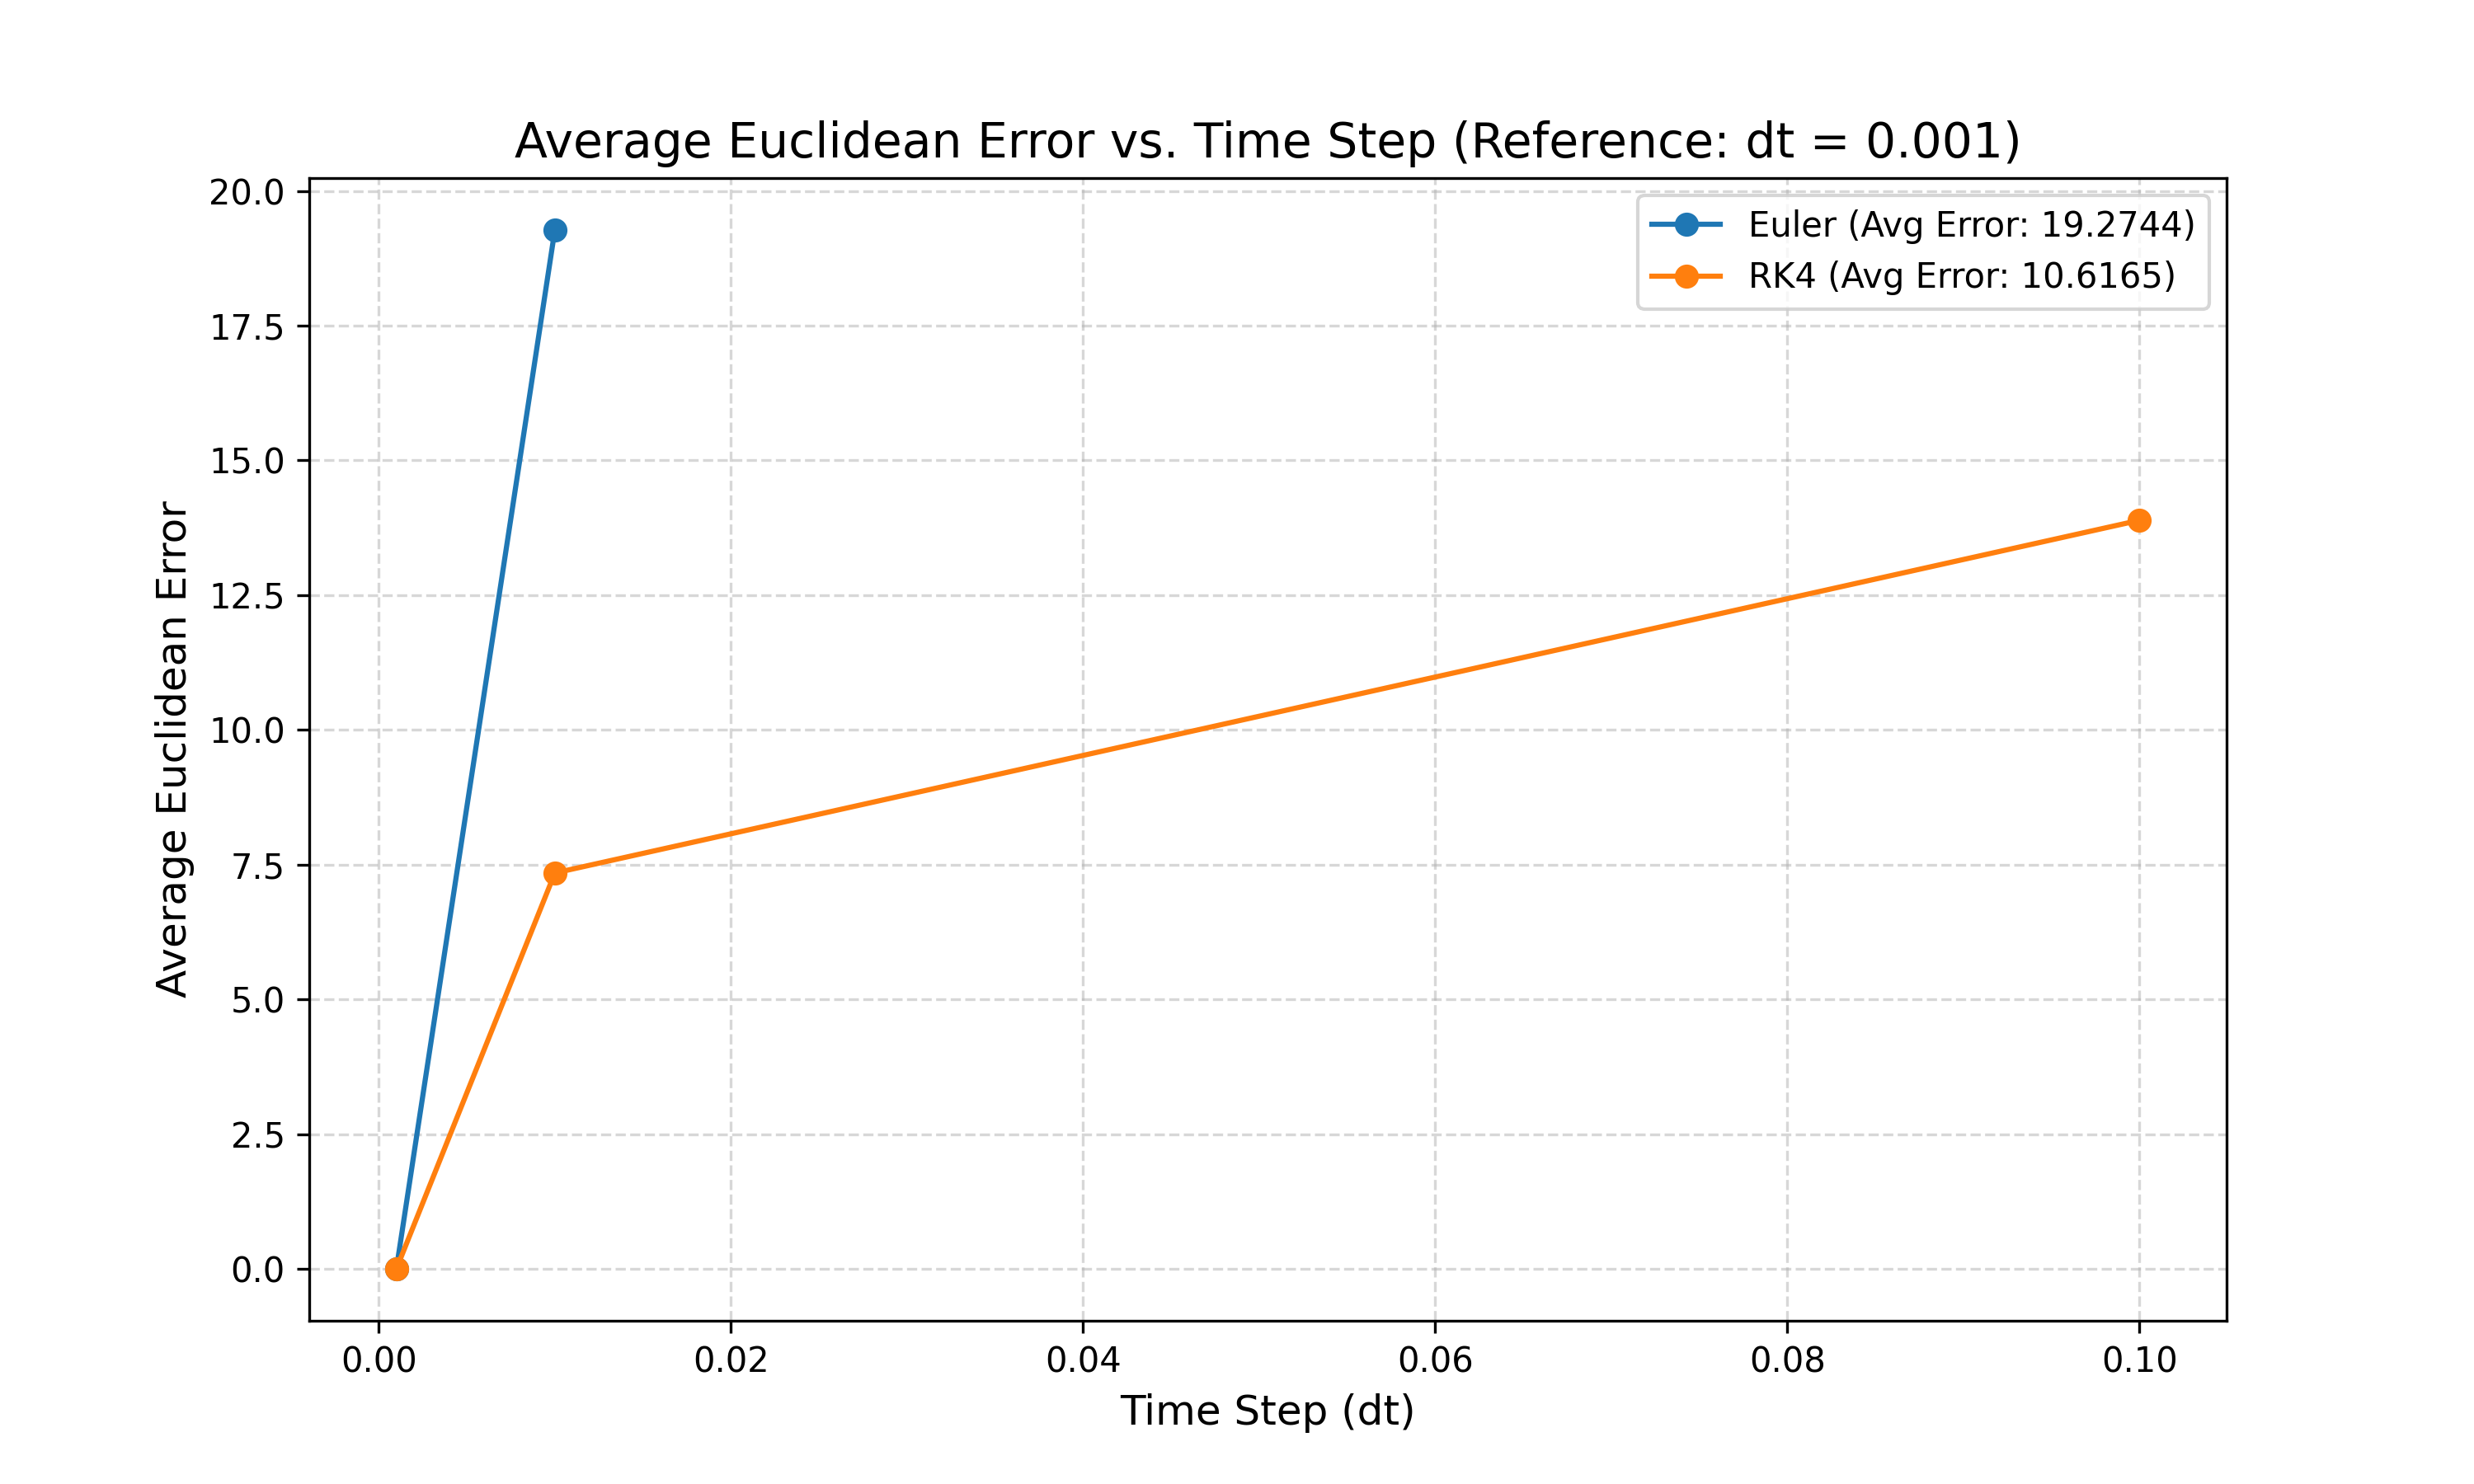
\includegraphics[width=1.0\linewidth]{images/error_comparison1.1.4.png} 
  \caption{Lorenz attractor error analysis with initial state (1.0,1.0,1.0) and time step (0.001, 0.01, 0.1), and total simulation time of 40 seconds,  For $\Delta t > 0.01$, the solution is not stable enough to reliably reproduce the attractor shape\cite{youngaryanLorenzPlot1.1.4_image}}
  \label{fig:error_comparison1.1.4}
\end{figure}

\begin{figure}[!ht]
  \centering
  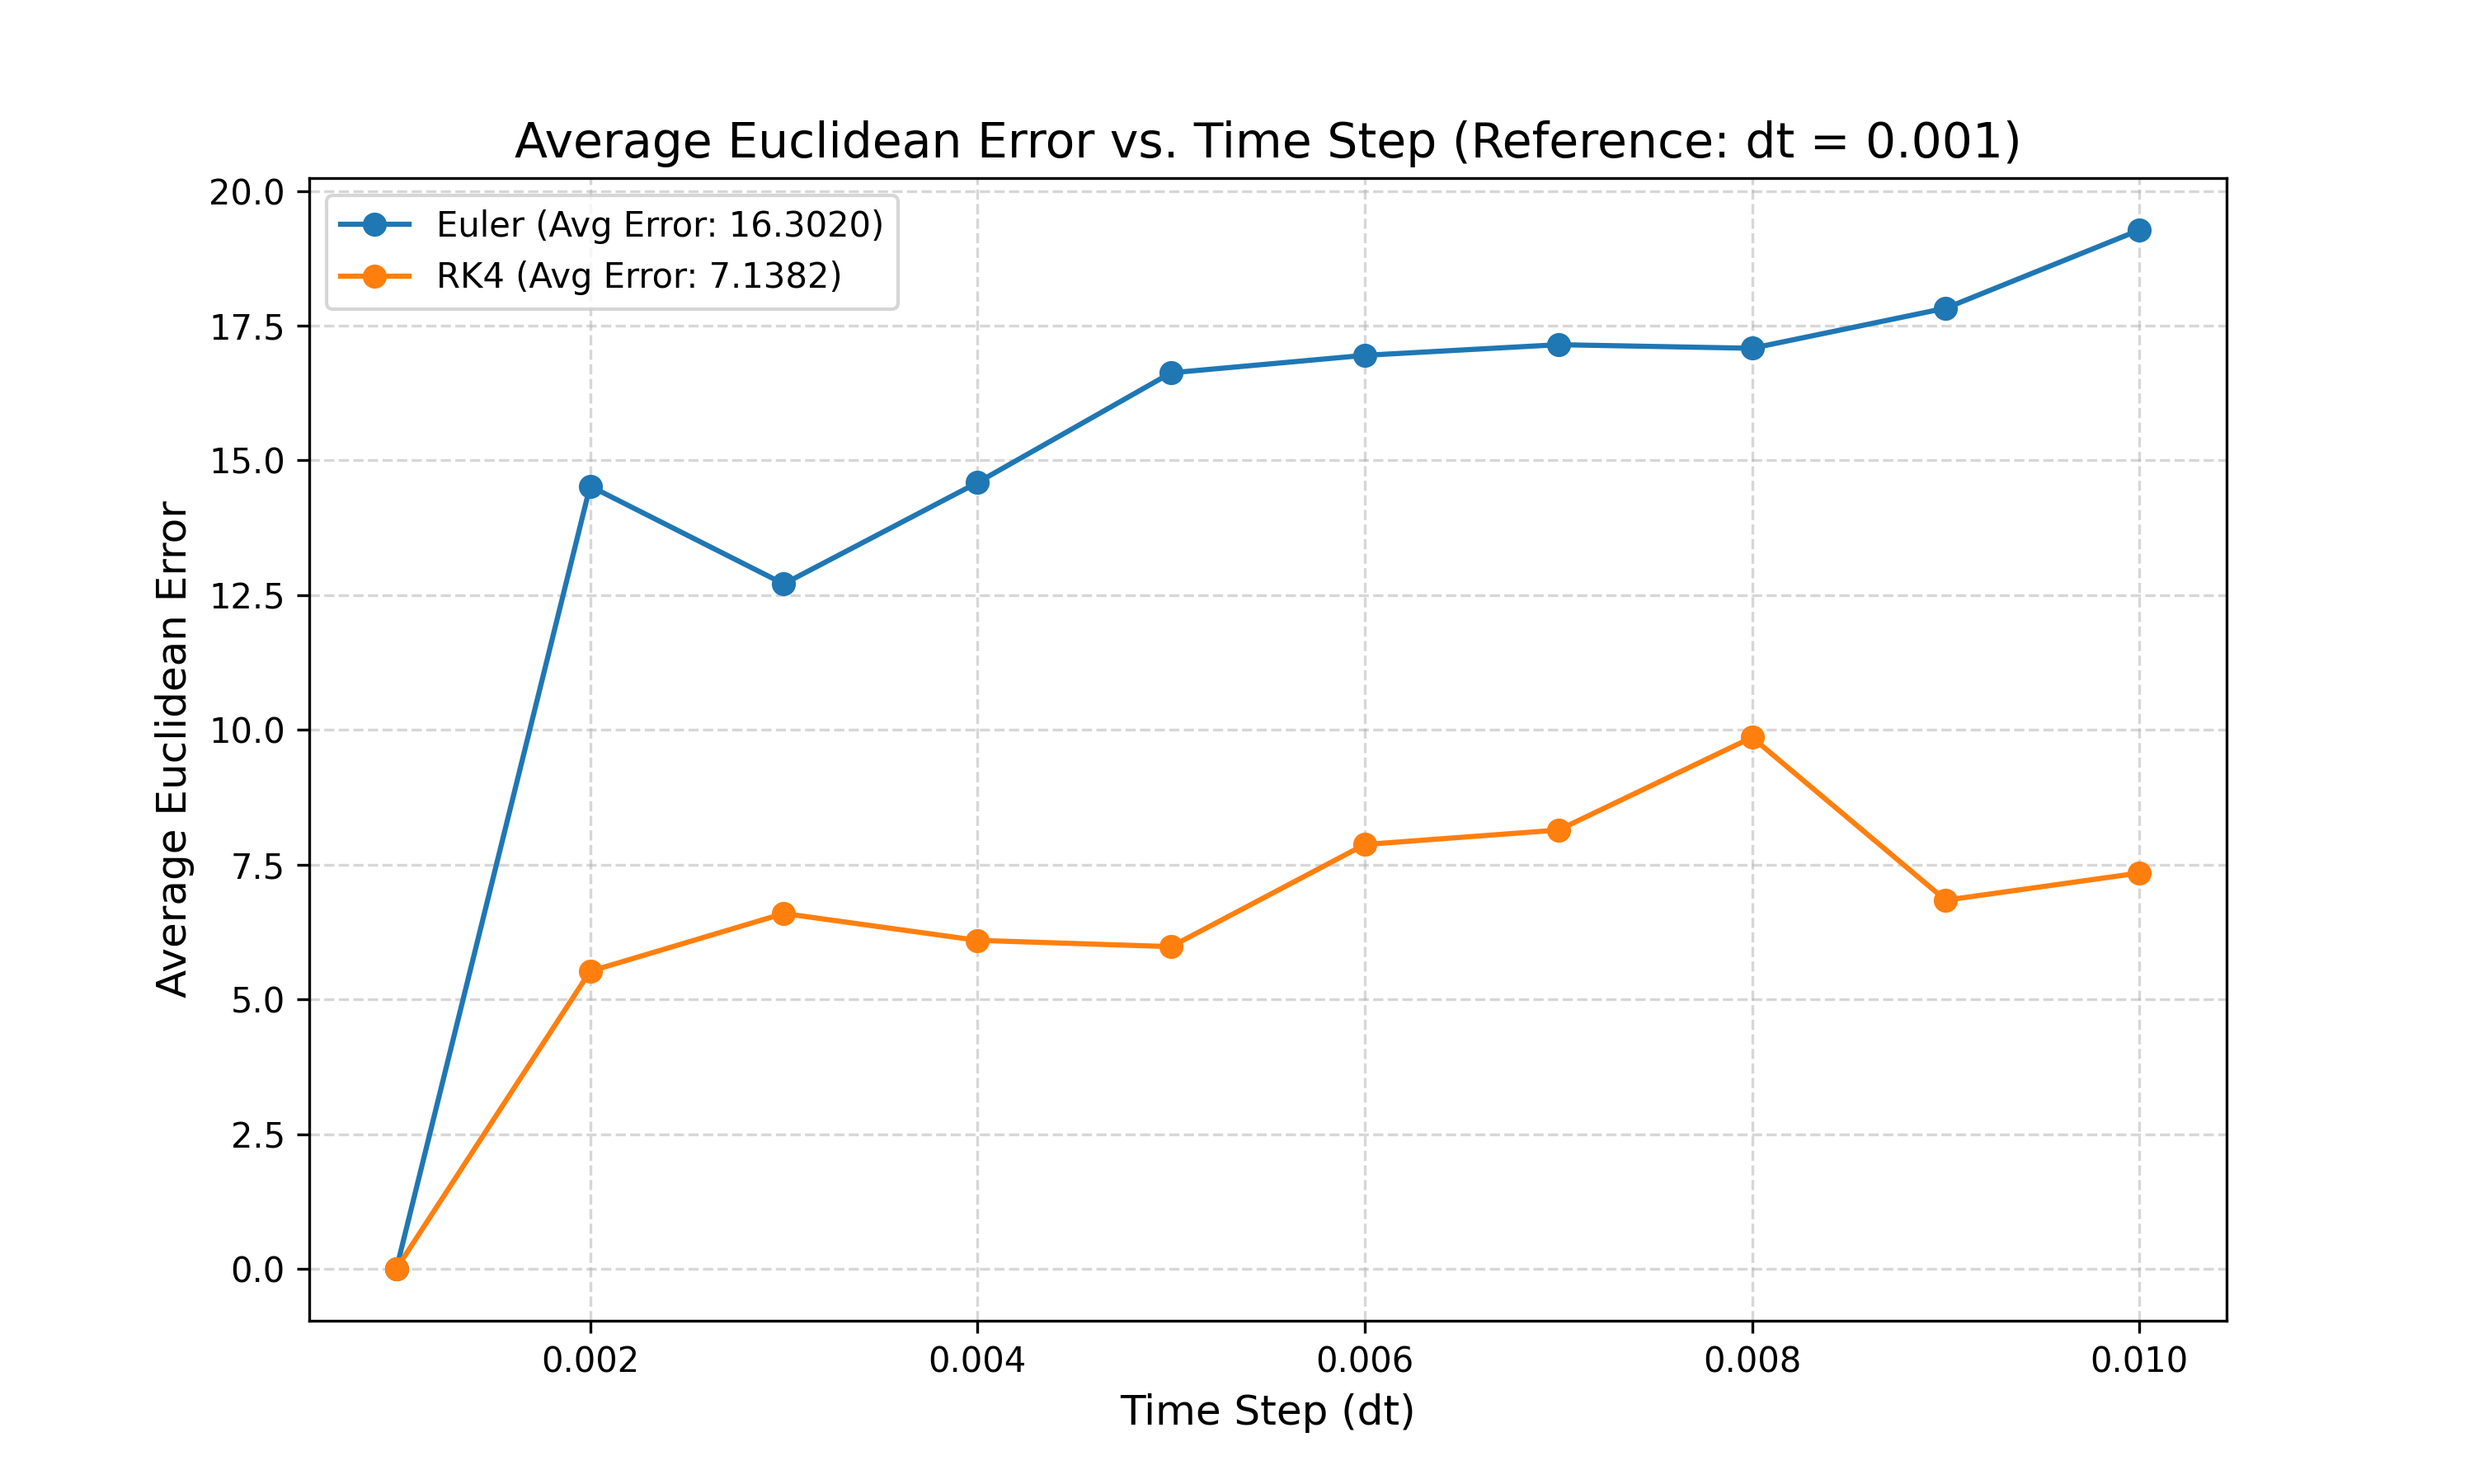
\includegraphics[width=0.9\linewidth]{images/error_comparison_same_times.png}
  \caption{Lorenz attractor error analysis with initial state \((1.0, 1.0, 1.0)\), 1000 different time steps between \((0.0001 and 0.001)\), and a total simulation time of 40 seconds. this experiment is to compare the mean error of the two methods\cite{youngaryanLorenzError1.1.4_image}.}
  \label{fig:error_comparison_same_times}
\end{figure}





\begin{figure}[!ht]
  \centering
  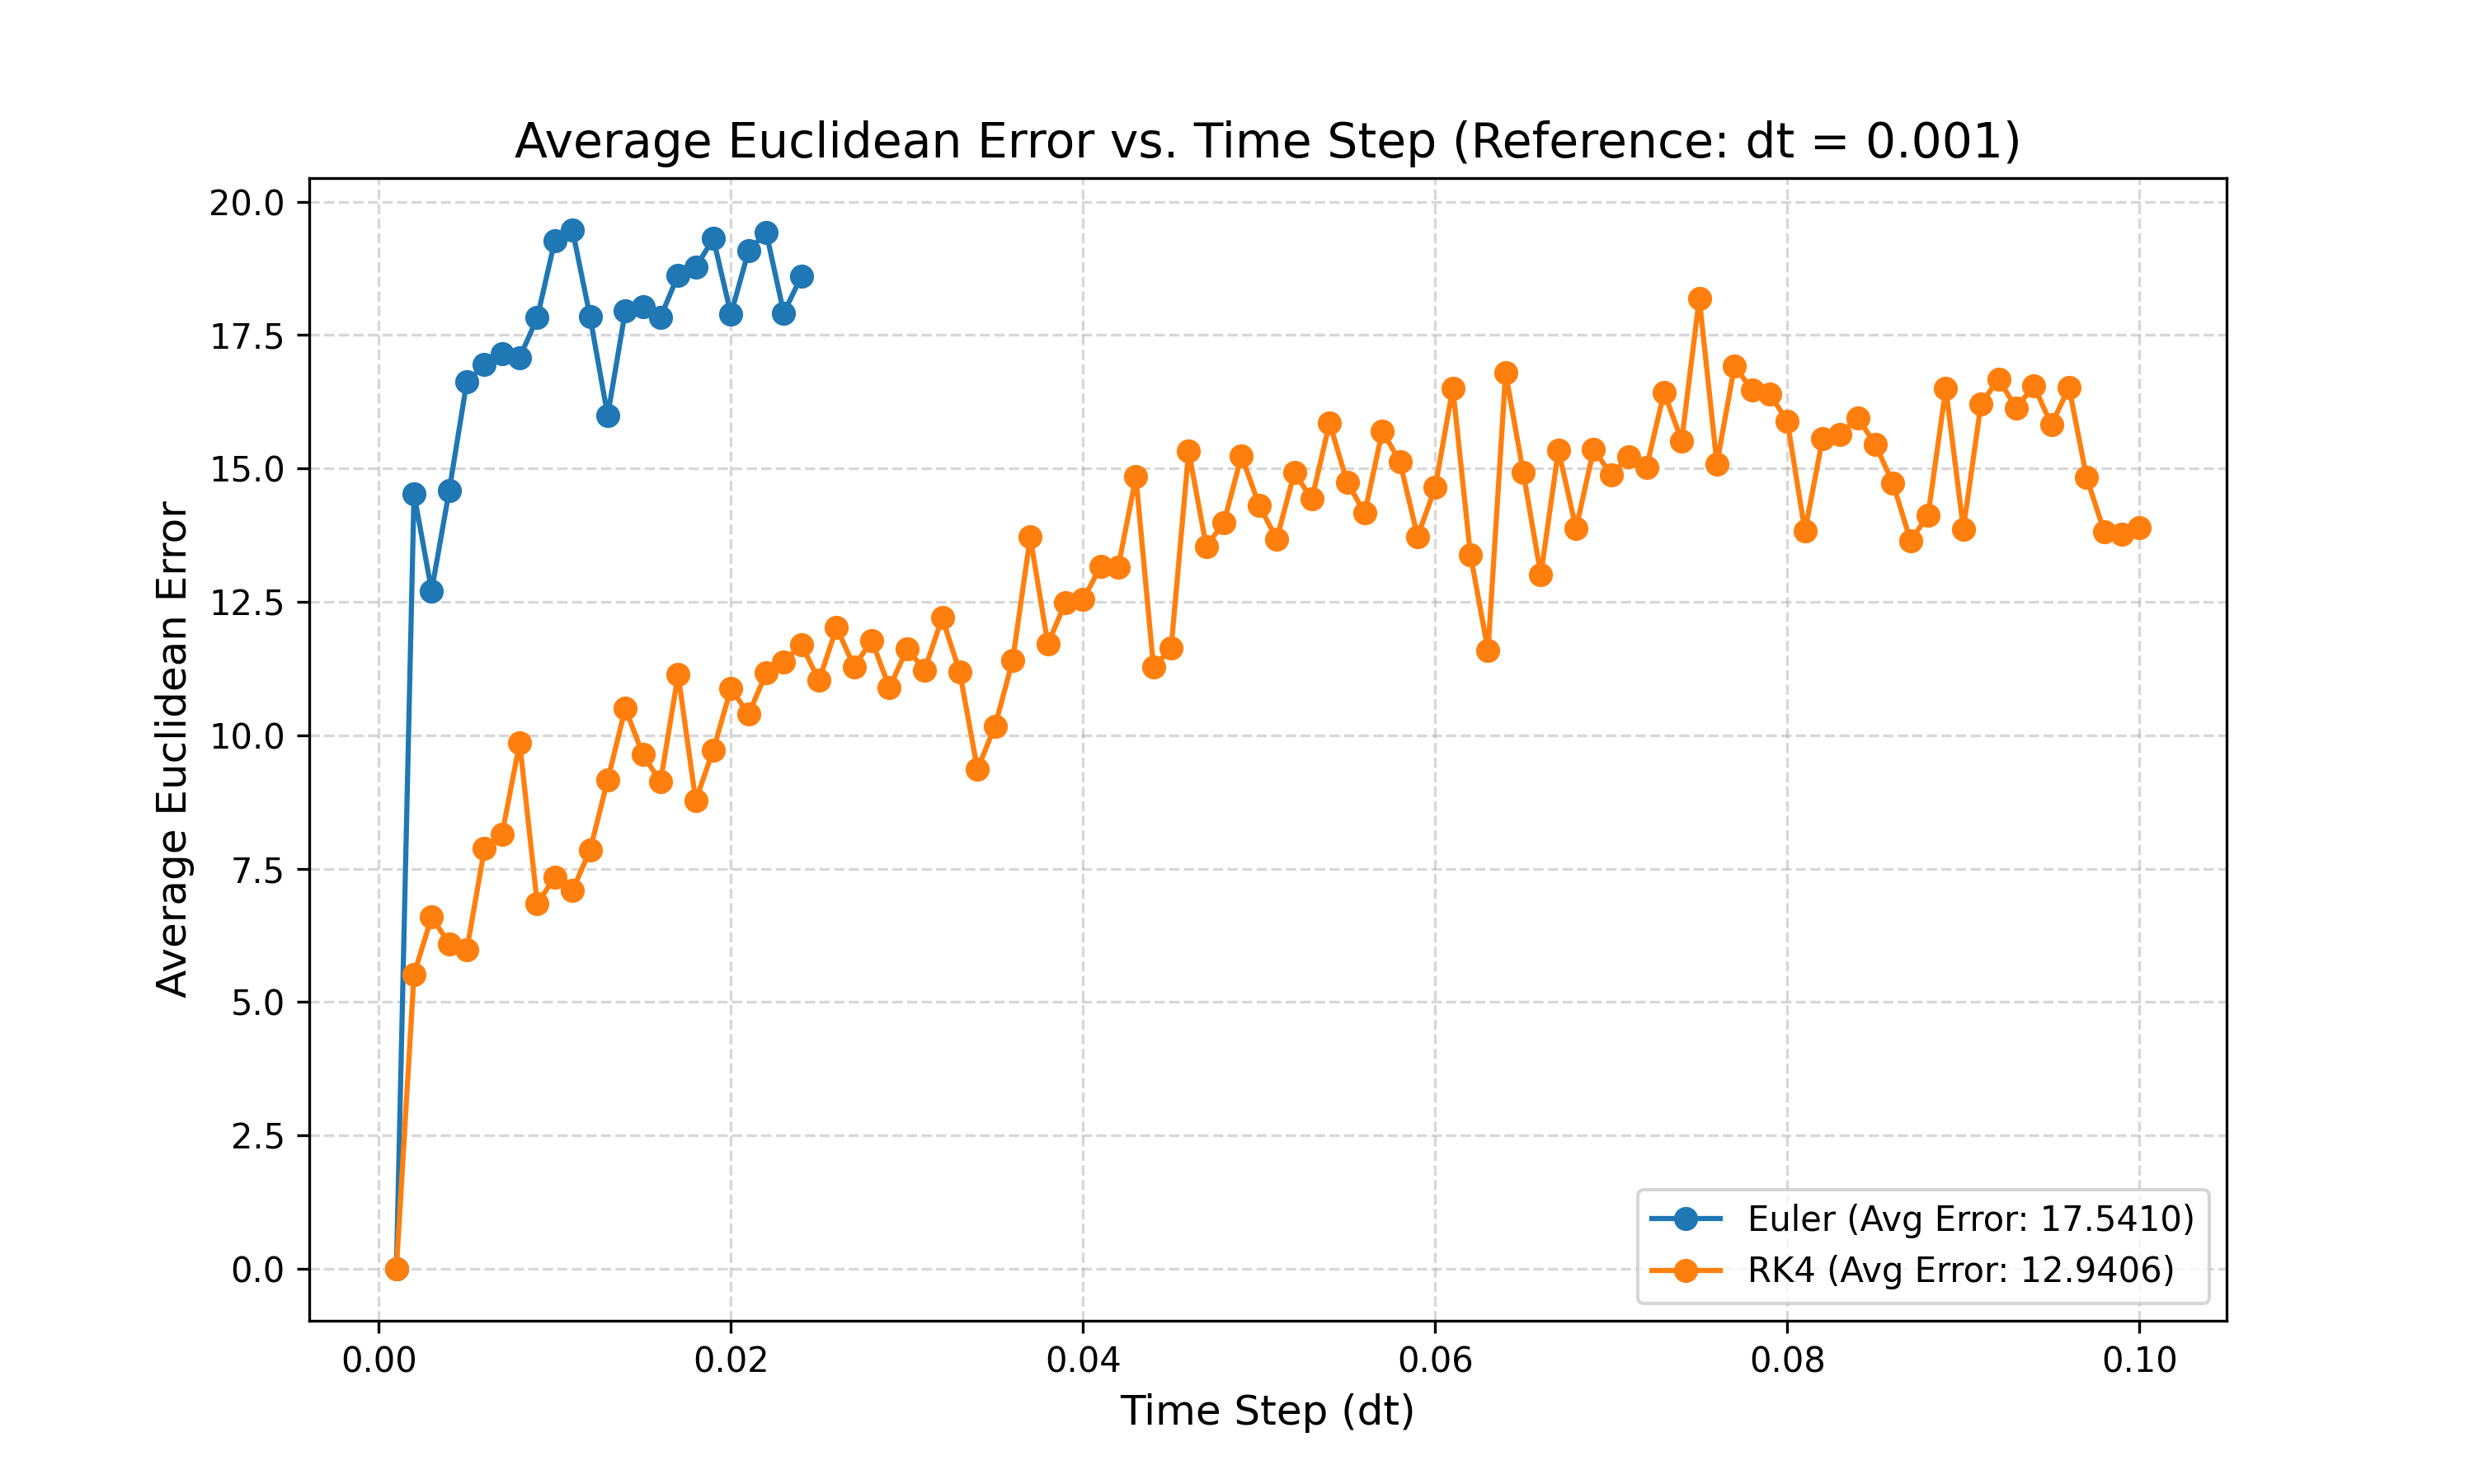
\includegraphics[width=0.9\linewidth]{images/error_comparison1000_114.png}
  \caption{Lorenz attractor error analysis with initial state \((1.0, 1.0, 1.0)\), using 1000 different time steps between \(10^{-3}\) and \(10^{-1}\), and a total simulation time of 40 seconds. For \(\Delta t > 0.025\), the Euler solution is not stable enough to reliably reproduce the attractor shape.
  \cite{youngaryanLorenzError1.1.41000_image}.}
  \label{fig:lorenz_error1000}
\end{figure}



\begin{figure}[!ht]
  \centering
  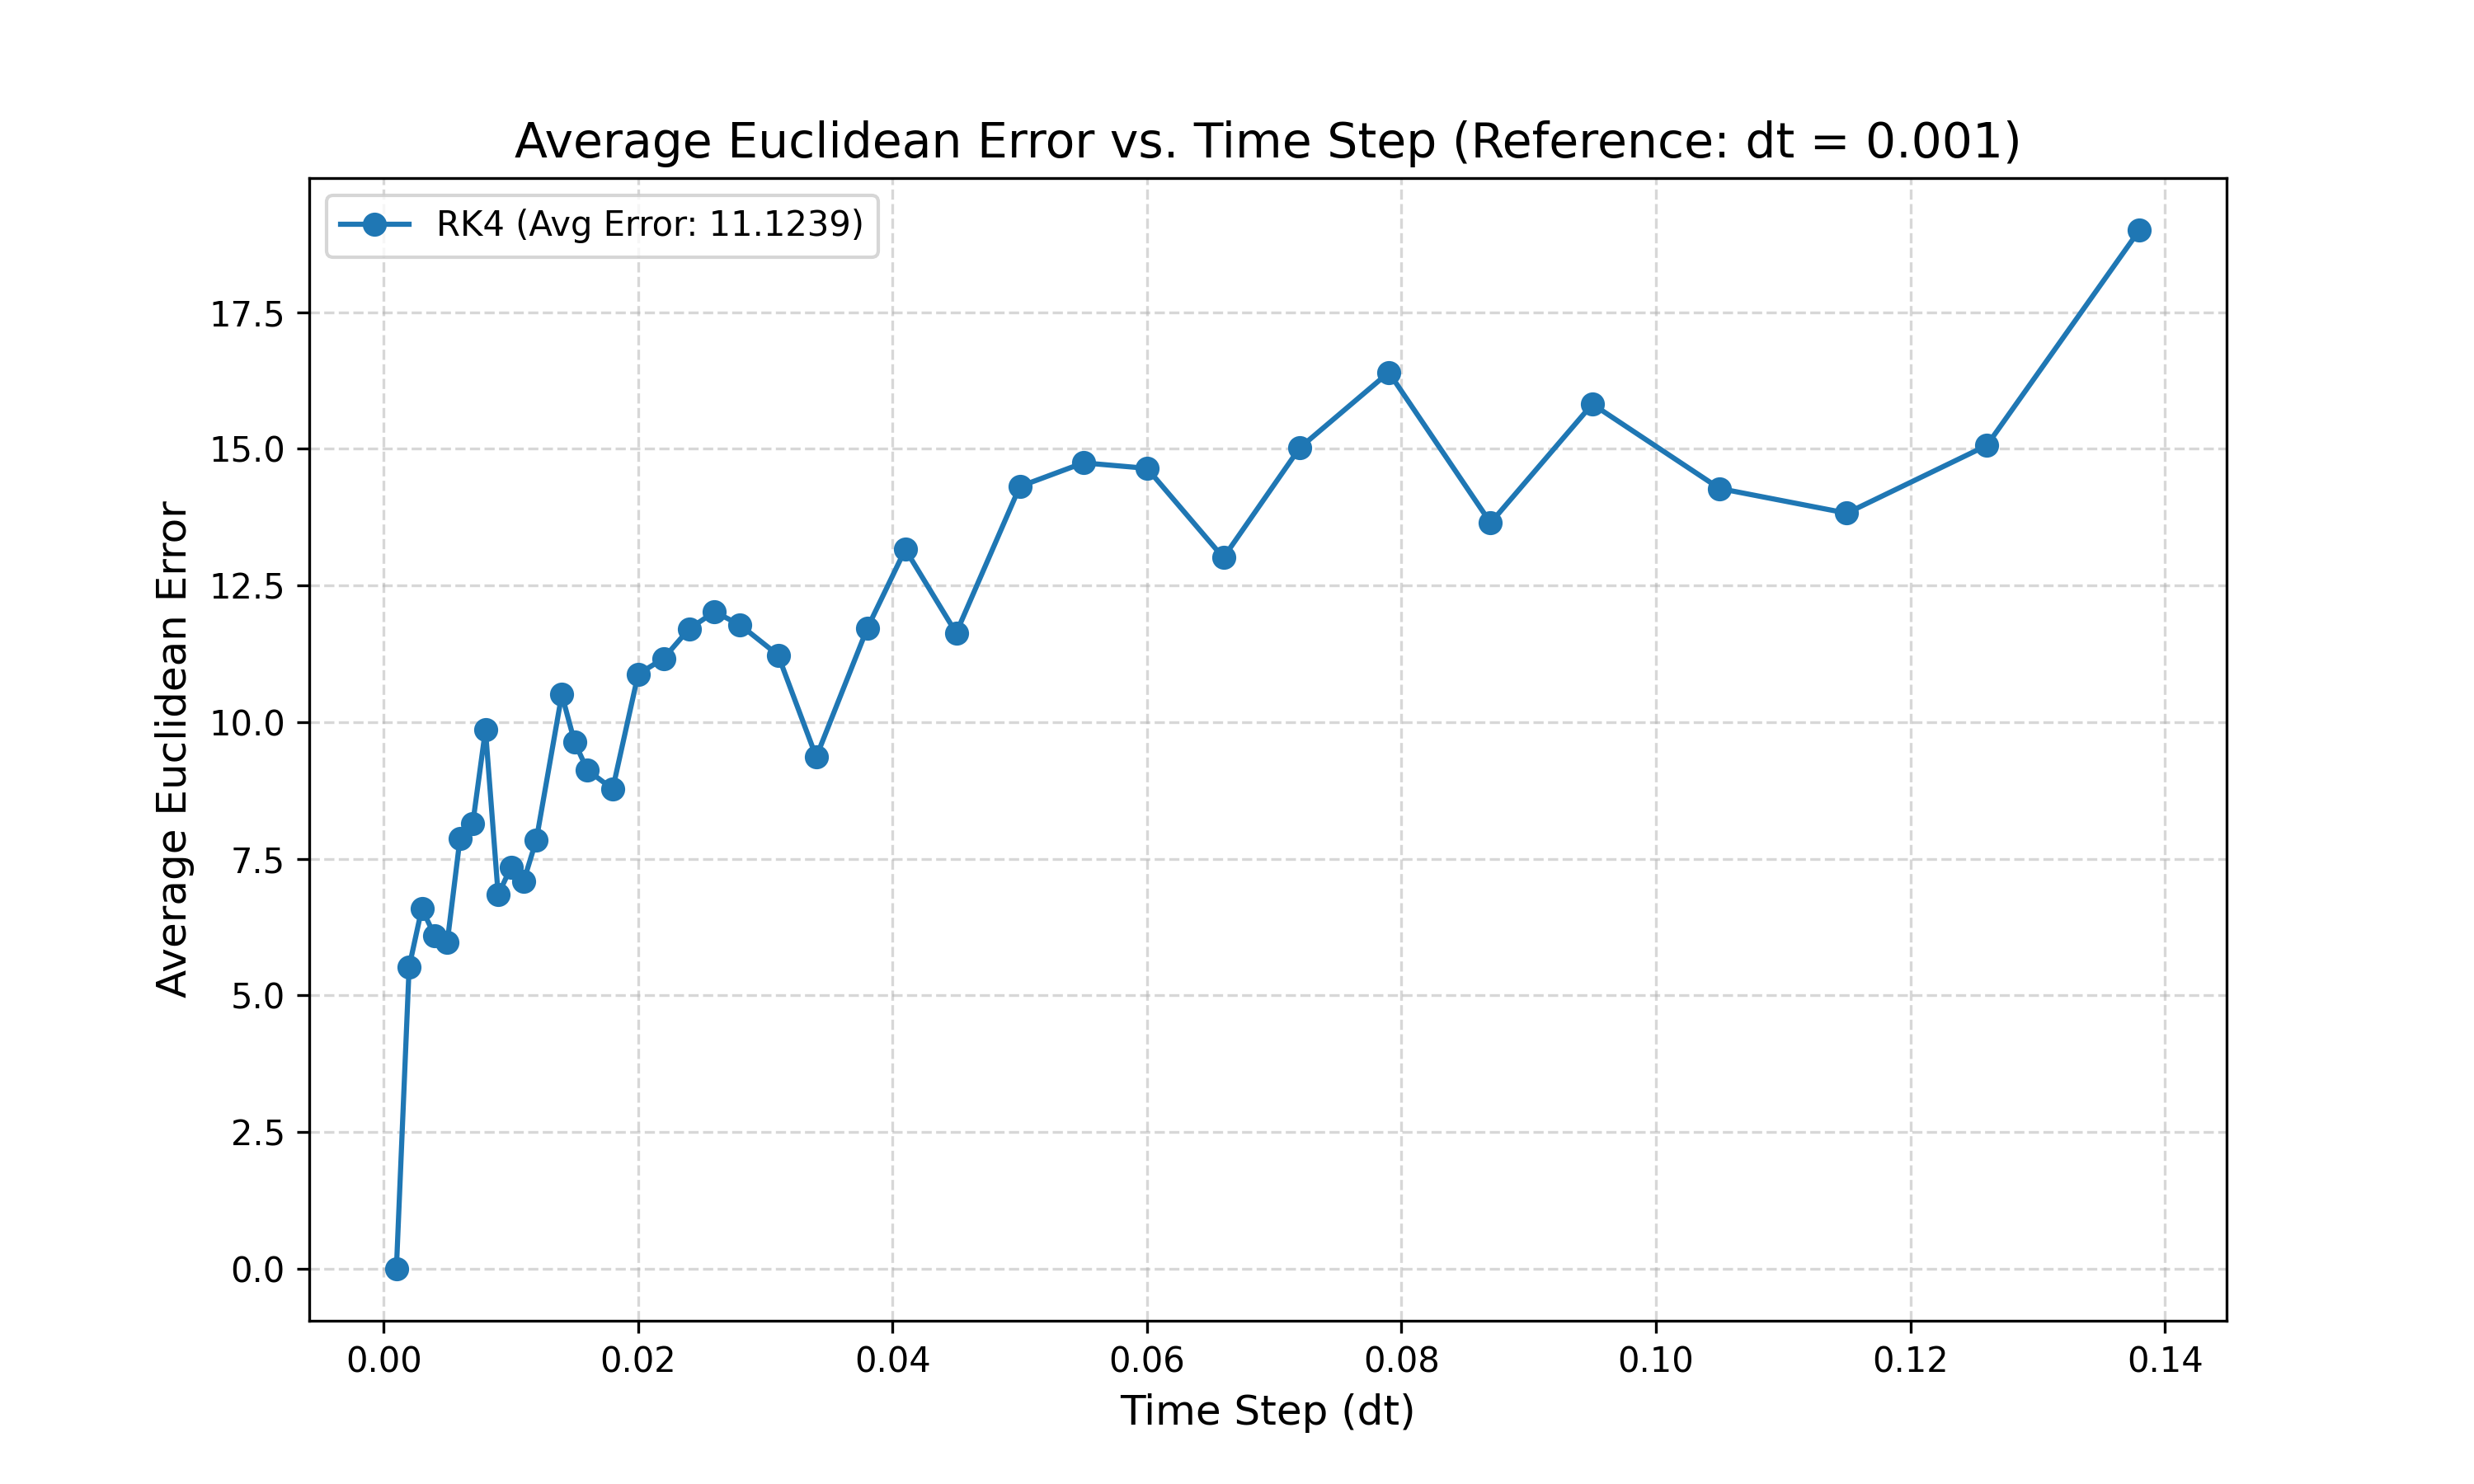
\includegraphics[width=0.9\linewidth]{images/error_comparison_rk4_stable_0.13.png}
  \caption{Lorenz attractor error analysis with initial state \((1.0, 1.0, 1.0)\), using 100 different time steps between \(10^{-3}\) and \(10^{1}\), and a total simulation time of 40 seconds. For \(\Delta t < 0.14\), the RK4 solution is stable enough to  reproduce the attractor shape. \cite{youngaryanerror_comparison_rk4_stable_0.13sCode}.}
  \label{fig:error_comparison_rk4_stable_0.13}
\end{figure}

\begin{figure}[!ht]
  \centering
  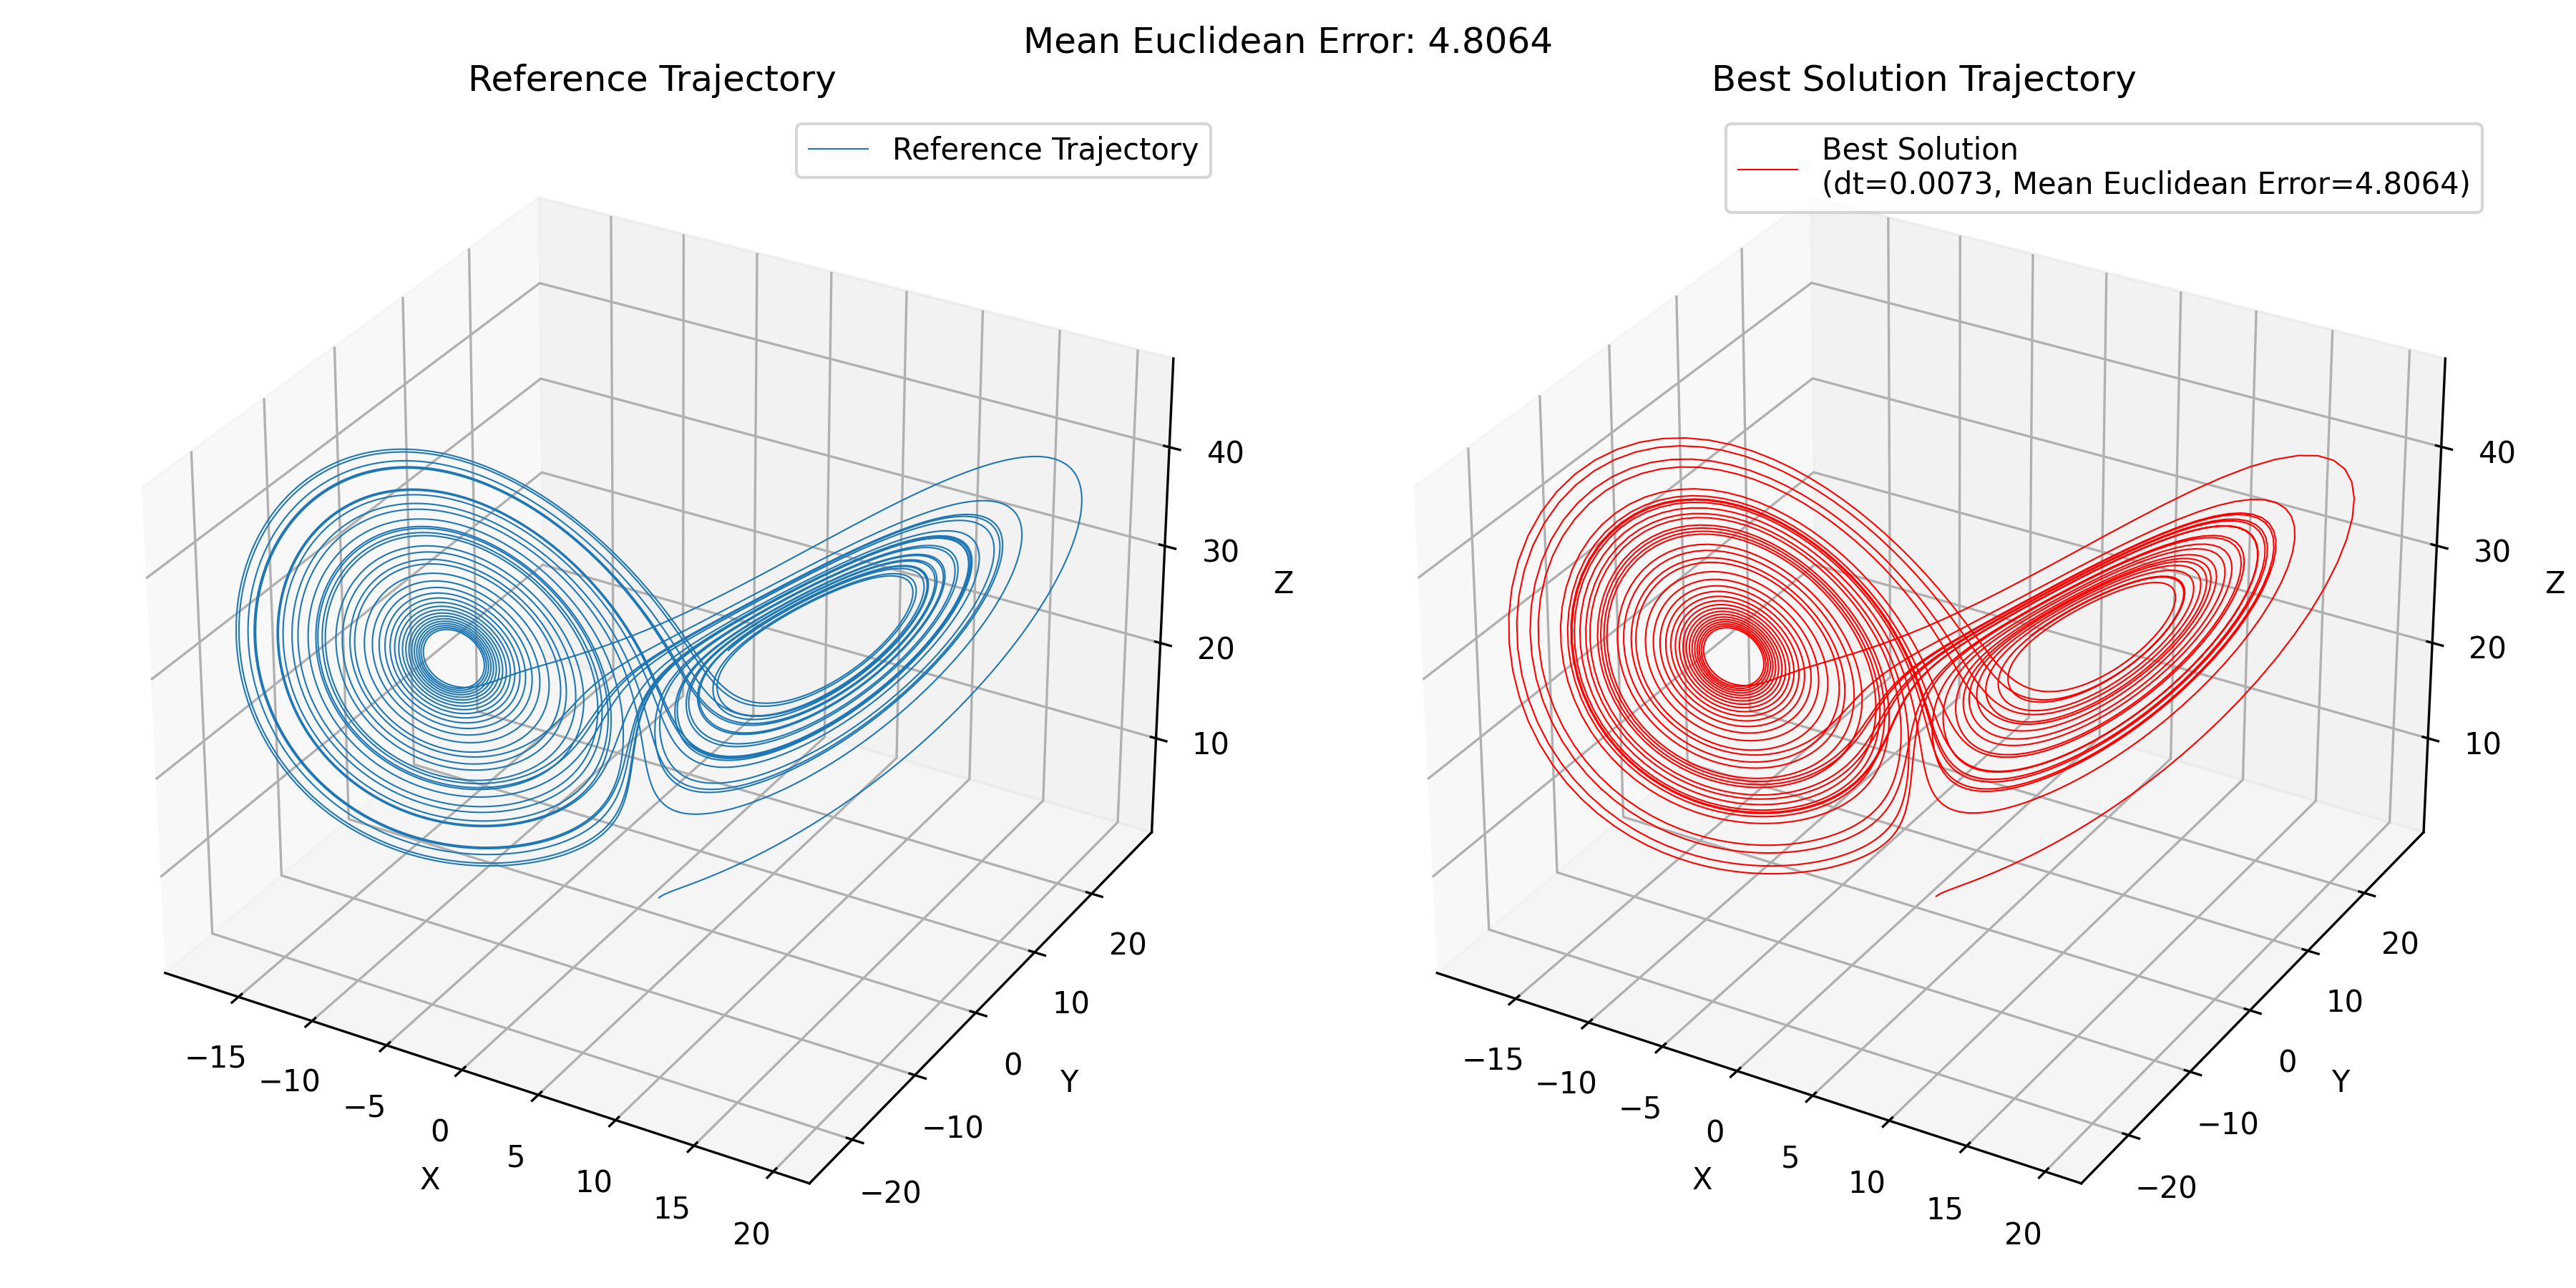
\includegraphics[width=0.9\linewidth]{images/optuna_lorenz_3d.png}
  \caption{Comparison between reference system with \(\Delta t = 0.001\) and a less computationally expensive system with step size of \(\Delta t = 0.0073\), for this I used Optuna \cite{akiba2019optuna} with 50 trials. the code is at \cite{youngaryanOptunaCode} and the image \cite{youngaryanoptunaComparisonImage}.}
  \label{fig:optuna_lorenz_3d}
\end{figure}


\begin{figure}[!ht]
  \centering
  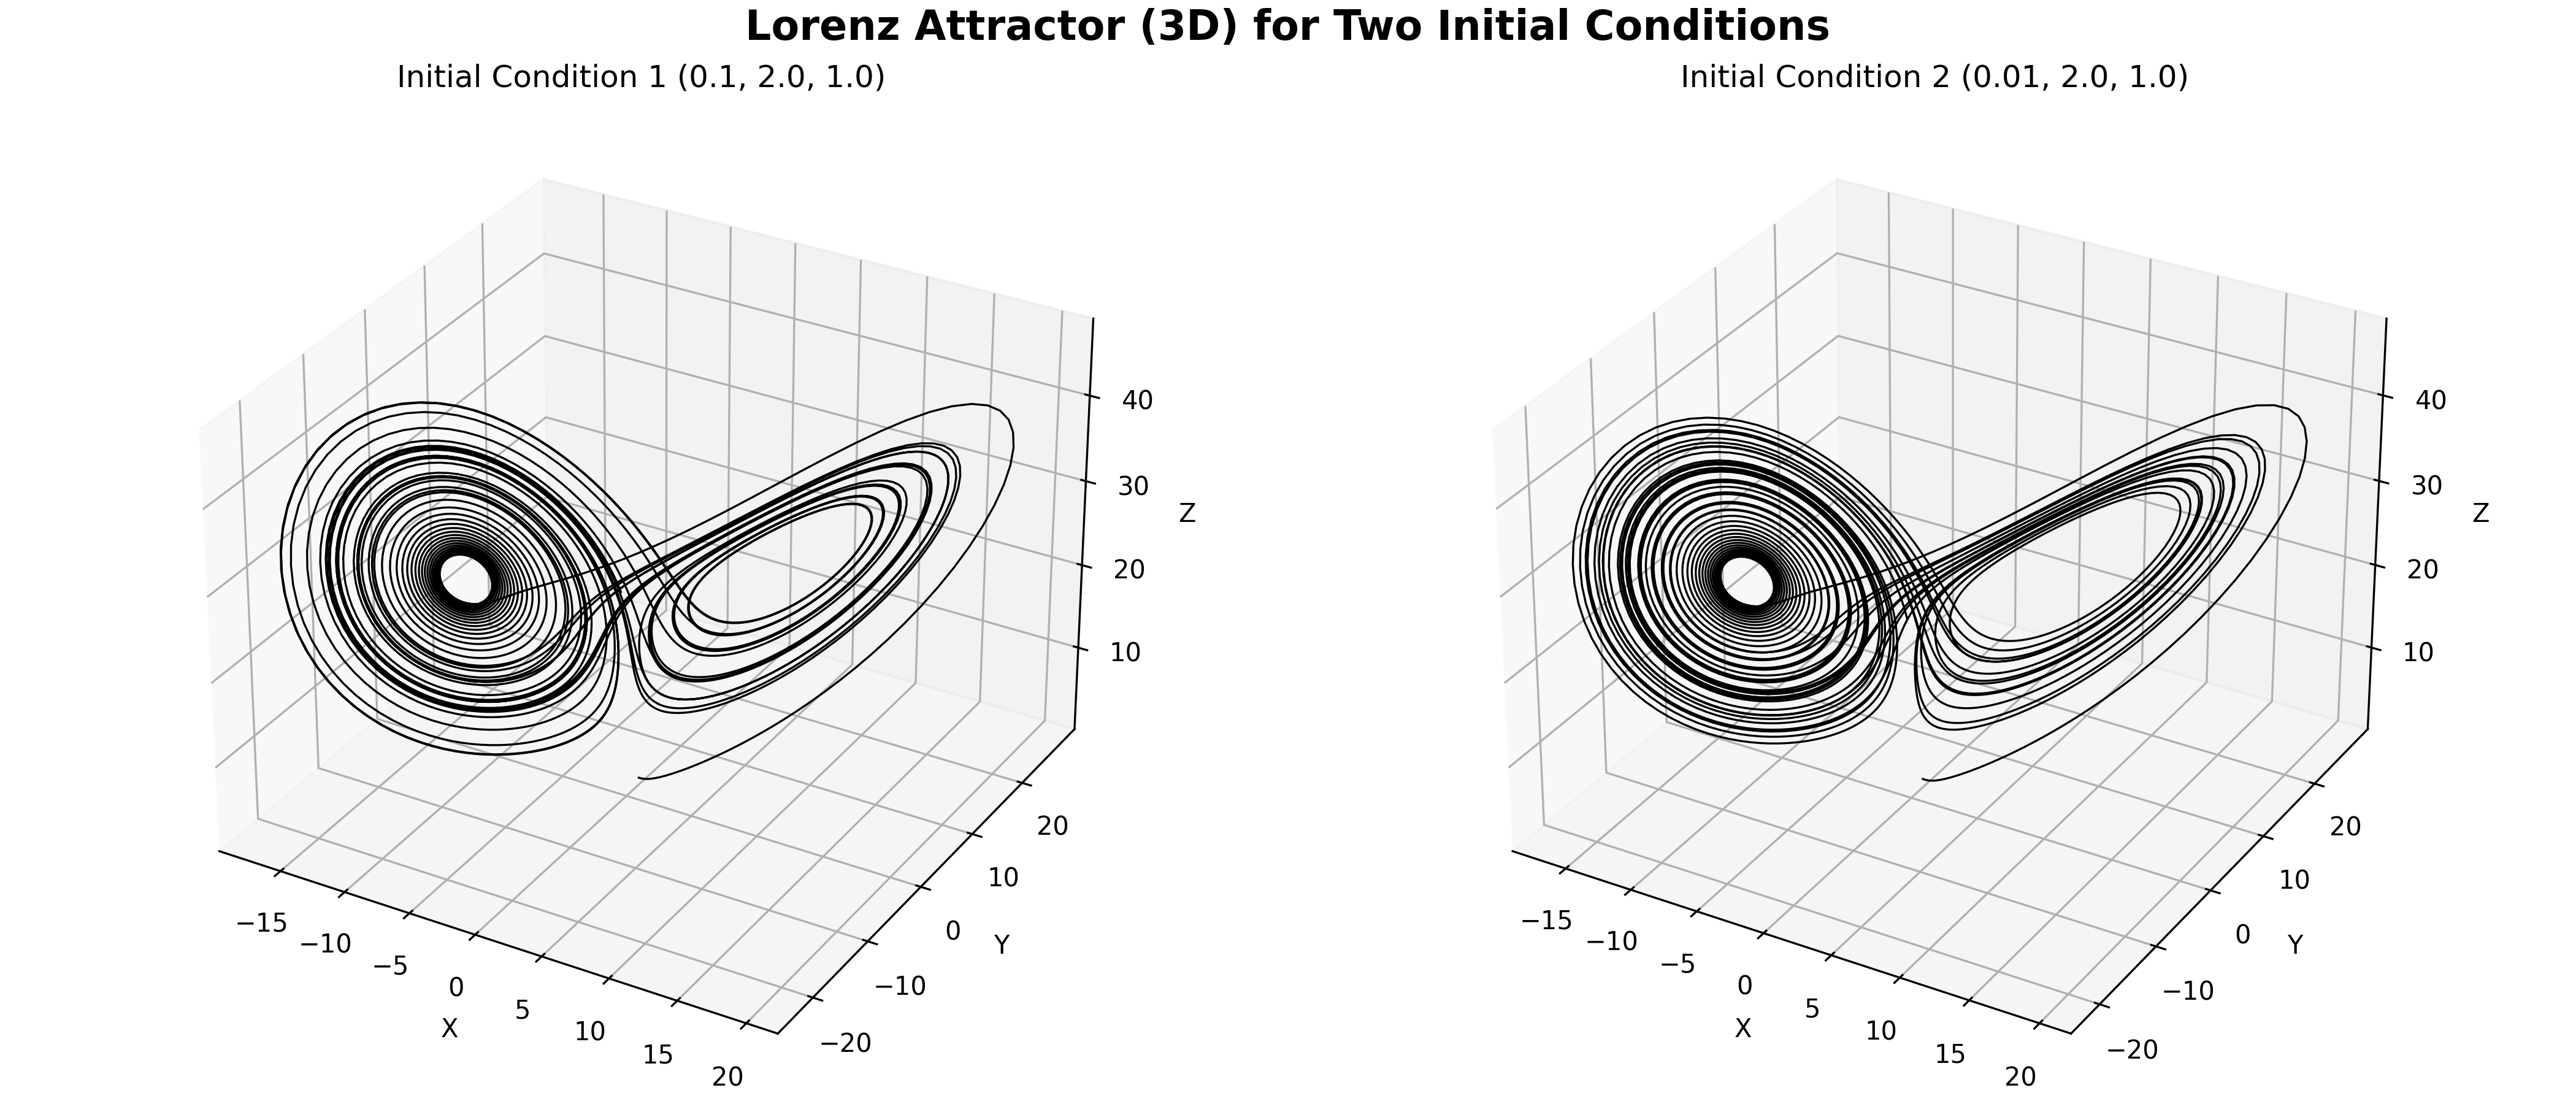
\includegraphics[width=0.9\linewidth]{images/two_initial_conditions_3d_separate.png}
  \caption{Comparison between two similar initial conditions of (0.01, 2.0, 1.0) and (0.1, 2.0, 1.0) and
  the time steps of $\Delta t = 0.0073$ to show the chaotic behavior of the system. the code is at \cite{youngaryantwo_initial_conditions_3d_separateICode} and the image \cite{youngaryantwo_initial_conditions_3d_separateImg}.}
  \label{fig:two_initial_conditions_3d_separate}
\end{figure}


\begin{figure}[!ht]
  \centering
  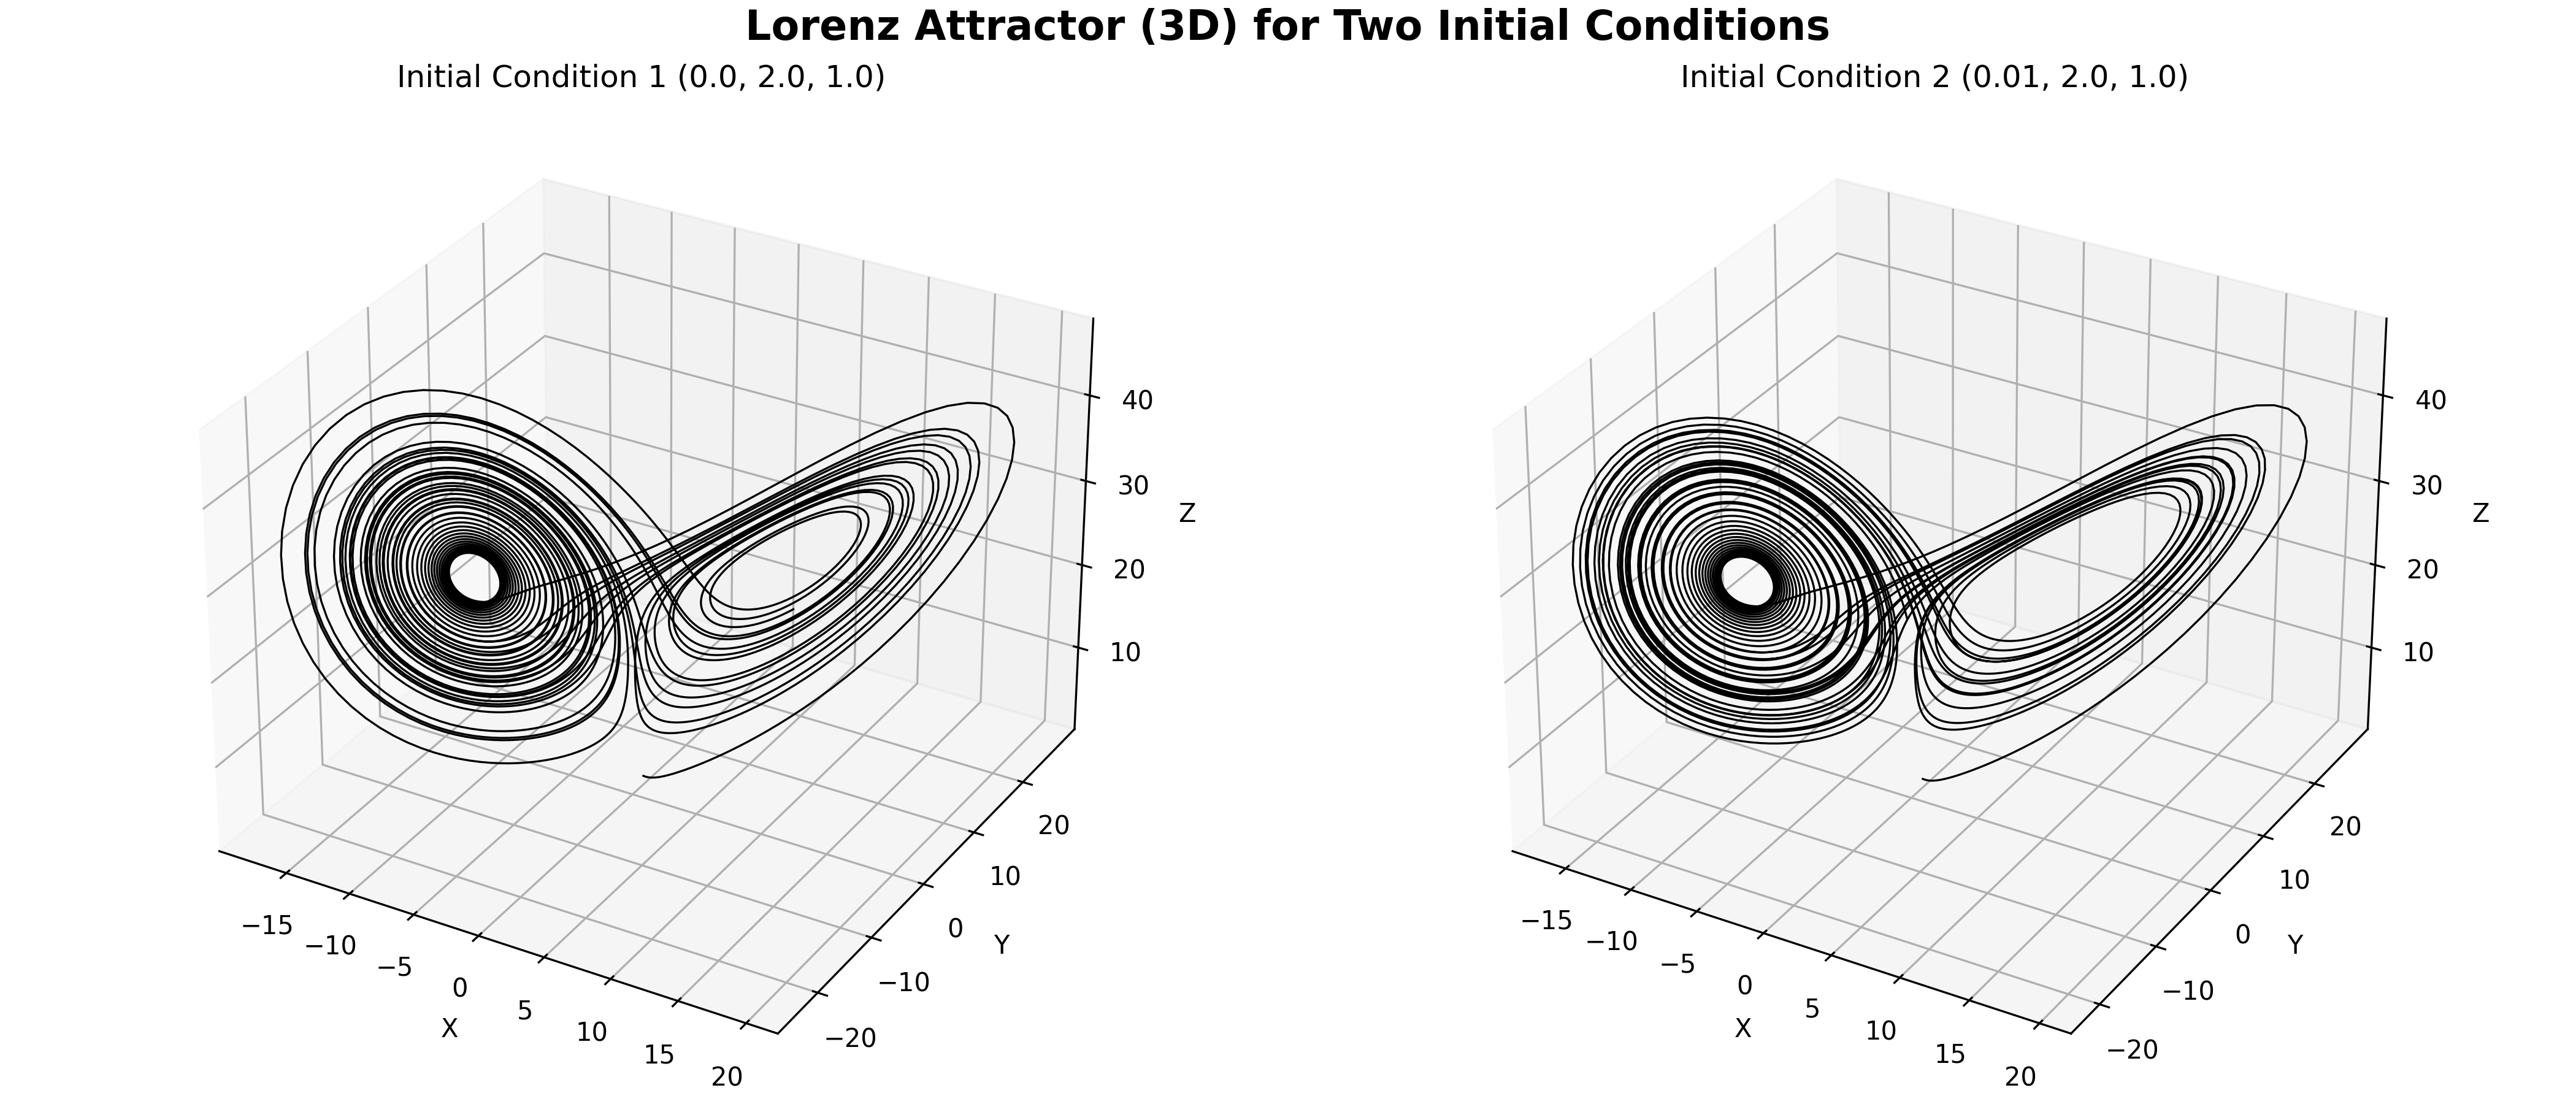
\includegraphics[width=0.9\linewidth]{images/two_initial_conditions_3d_separate_2.png}
  \caption{Comparison between two similar initial conditions of (0.0, 2.0, 1.0) and (0.1, 2.0, 1.0) and
the time steps of $\Delta t = 0.0073$ to show the chaotic behavior of the system. the code is at \cite{youngaryantwo_initial_conditions_3d_separateICode} and the image \cite{youngaryantwo_initial_conditions_3d_2separateICode}.}
  \label{fig:two_initial_conditions_3d_separate_2}
\end{figure}

\begin{figure}[!ht]
  \centering
  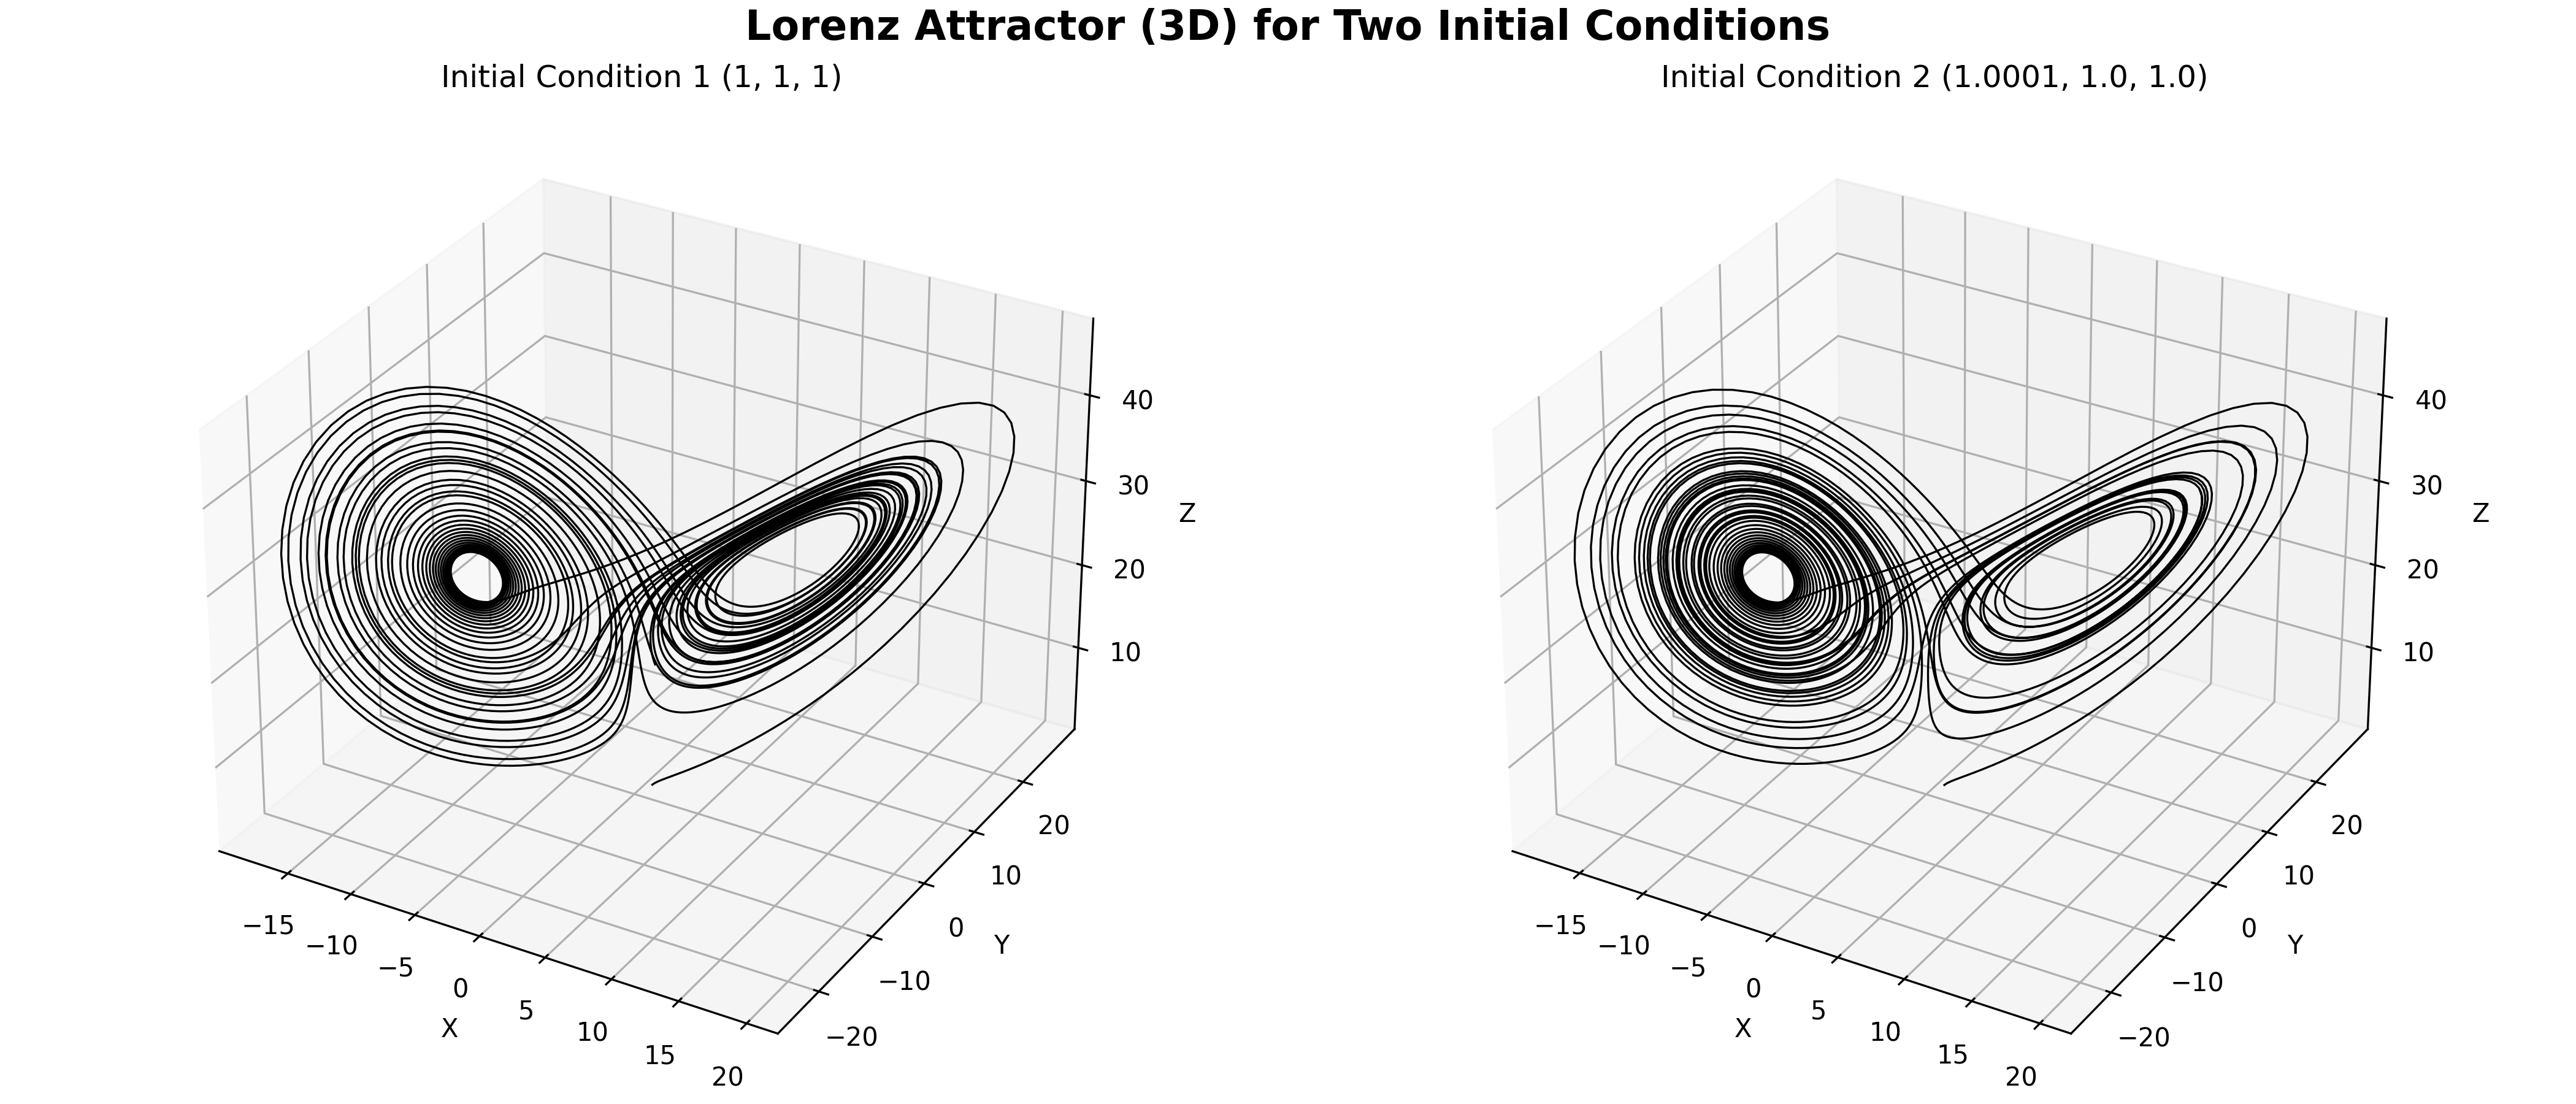
\includegraphics[width=0.9\linewidth]{images/two_initial_conditions_3d_separate_3.png}
  \caption{Comparison between two similar initial conditions of (1.0, 1.0, 1.0) and (1.0001, 1.0, 1.0) and
the time steps of$\Delta t = 0.0073$ to show the chaotic behavior of the system. the code is at \cite{youngaryantwo_initial_conditions_3d_separateICode} and the image \cite{youngaryantwo_initial_conditions_3d_3separateICode}.}
  \label{fig:two_initial_conditions_3d_separate_3}
\end{figure}



\begin{figure}[!ht]
  \centering
  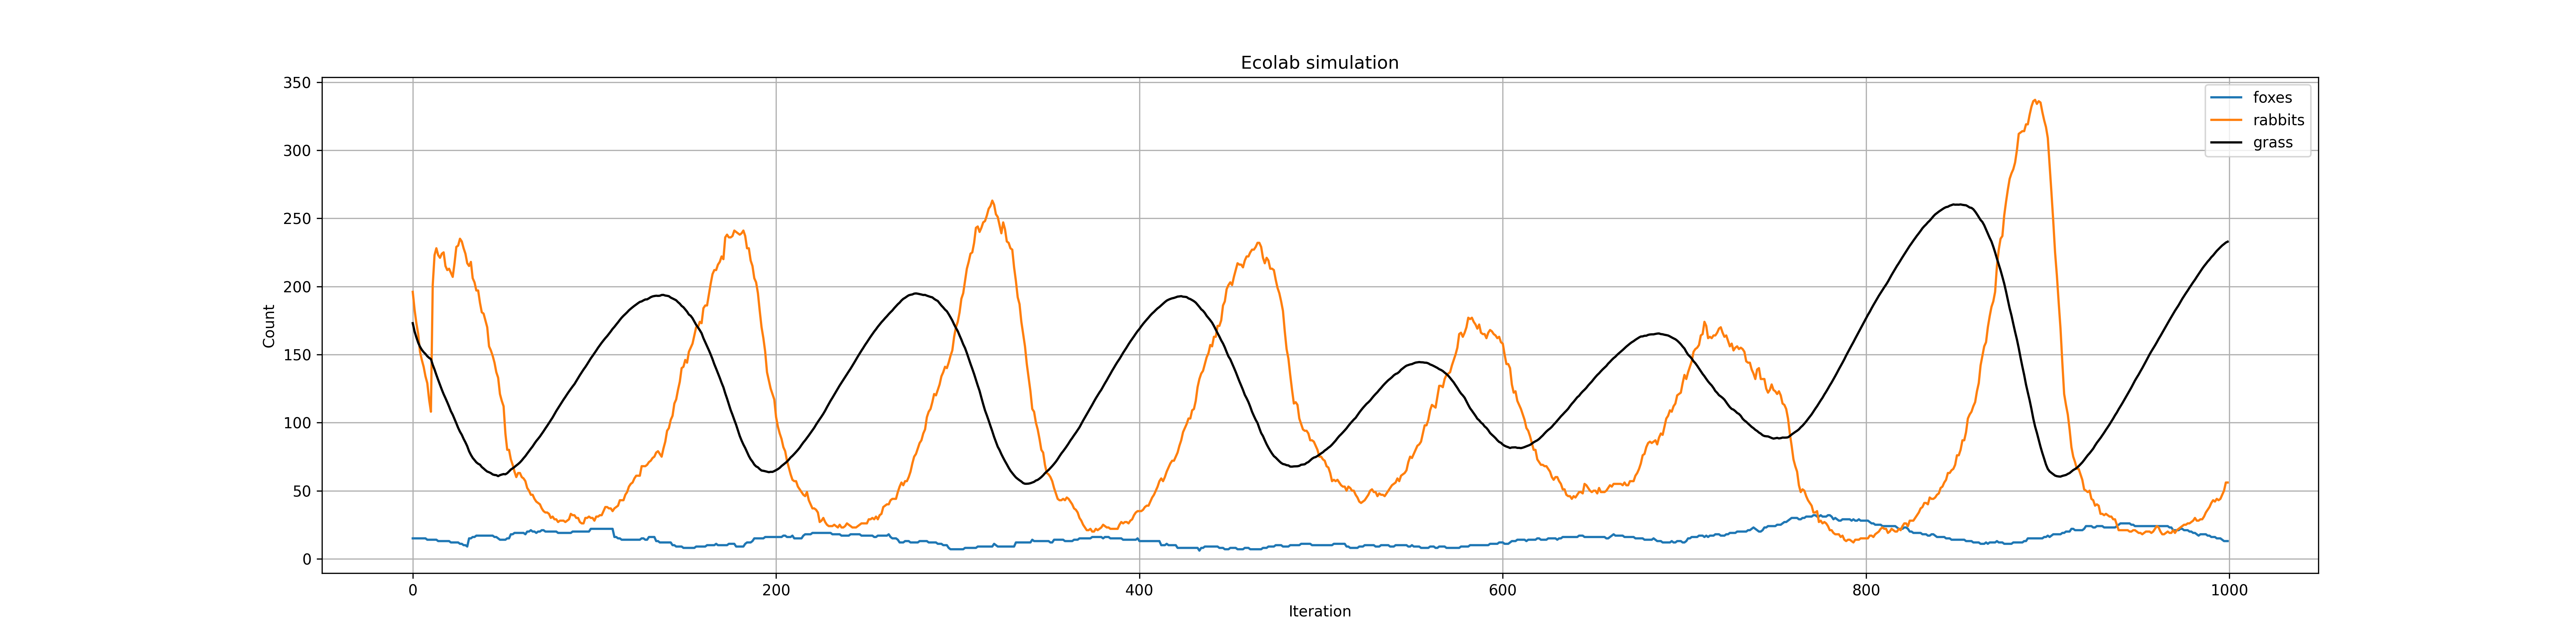
\includegraphics[width=0.9\linewidth]{images/Ecolab_simulation.png}
  \caption{Simulation of a prey-predator system with the following initial settings: \texttt{Environment(shape=[60,60], growrate=60, maxgrass=50, startgrass=1)}, \texttt{Nrabbits = 200}, \texttt{Nfoxes = 15}. Rabbits are initialized with \texttt{speed=1}, \texttt{vision=5}, \texttt{breedfreq=10}, \texttt{breedfood=10}, and \texttt{maxage=40}. Foxes are initialized with \texttt{speed=3}, \texttt{vision=7}, \texttt{breedfreq=30}, \texttt{breedfood=20}, and \texttt{maxage=80}. See \cite{youngaryantwo_initial_conditions_3d_separateICode} for code and \cite{youngaryantwo_initial_conditions_3d_3separateICode} for the source image.}
  \label{fig:Ecolab_pred_prey}
\end{figure}


\begin{figure}[!ht]
  \centering
  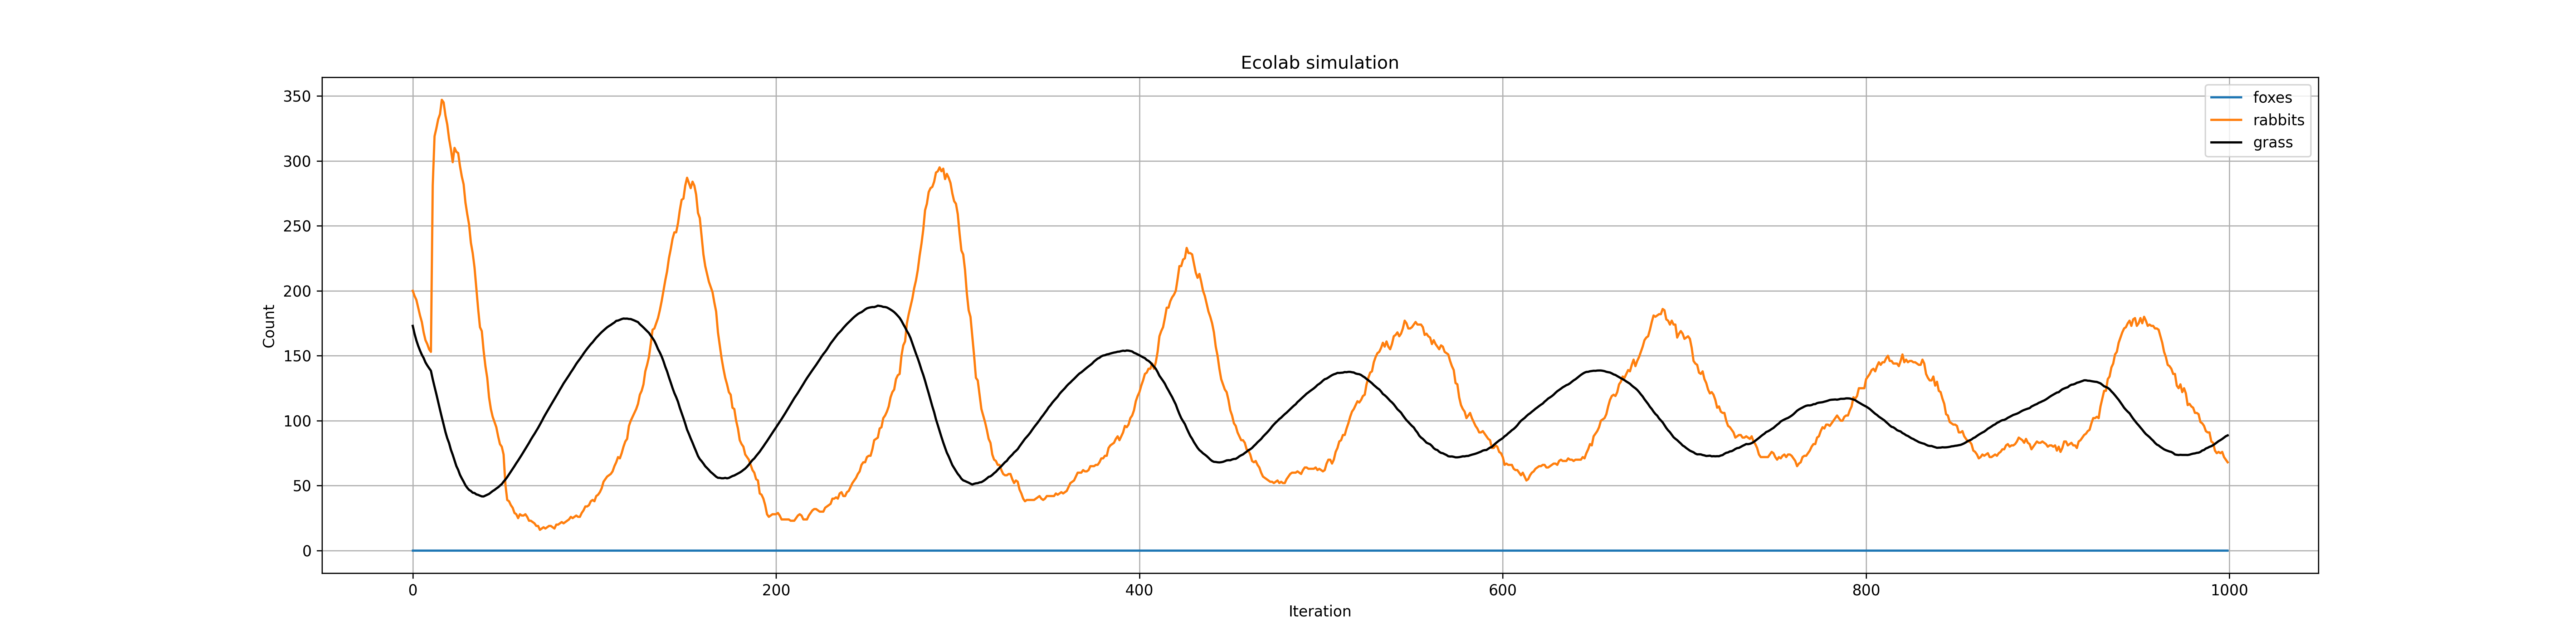
\includegraphics[width=0.9\linewidth]{images/Ecolab_simulation_no_foxes.png}
  \caption{Simulation of a prey-predator system with the following initial settings: \texttt{Environment(shape=[60,60], growrate=60, maxgrass=50, startgrass=1)}, \texttt{Nrabbits = 200}, \texttt{Nfoxes = 15}. Rabbits are initialized with \texttt{speed=1}, \texttt{vision=5}, \texttt{breedfreq=10}, \texttt{breedfood=10}, and \texttt{maxage=40}. And ero foxes. See \cite{youngaryantwo_initial_conditions_3d_separateICode} for code and \cite{youngaryantwo_initial_conditions_3d_3separateICode} for the source image.}
  \label{fig:Ecolab_pred_prey_no_foxes}
\end{figure}


\begin{figure}[!ht]
  \centering
  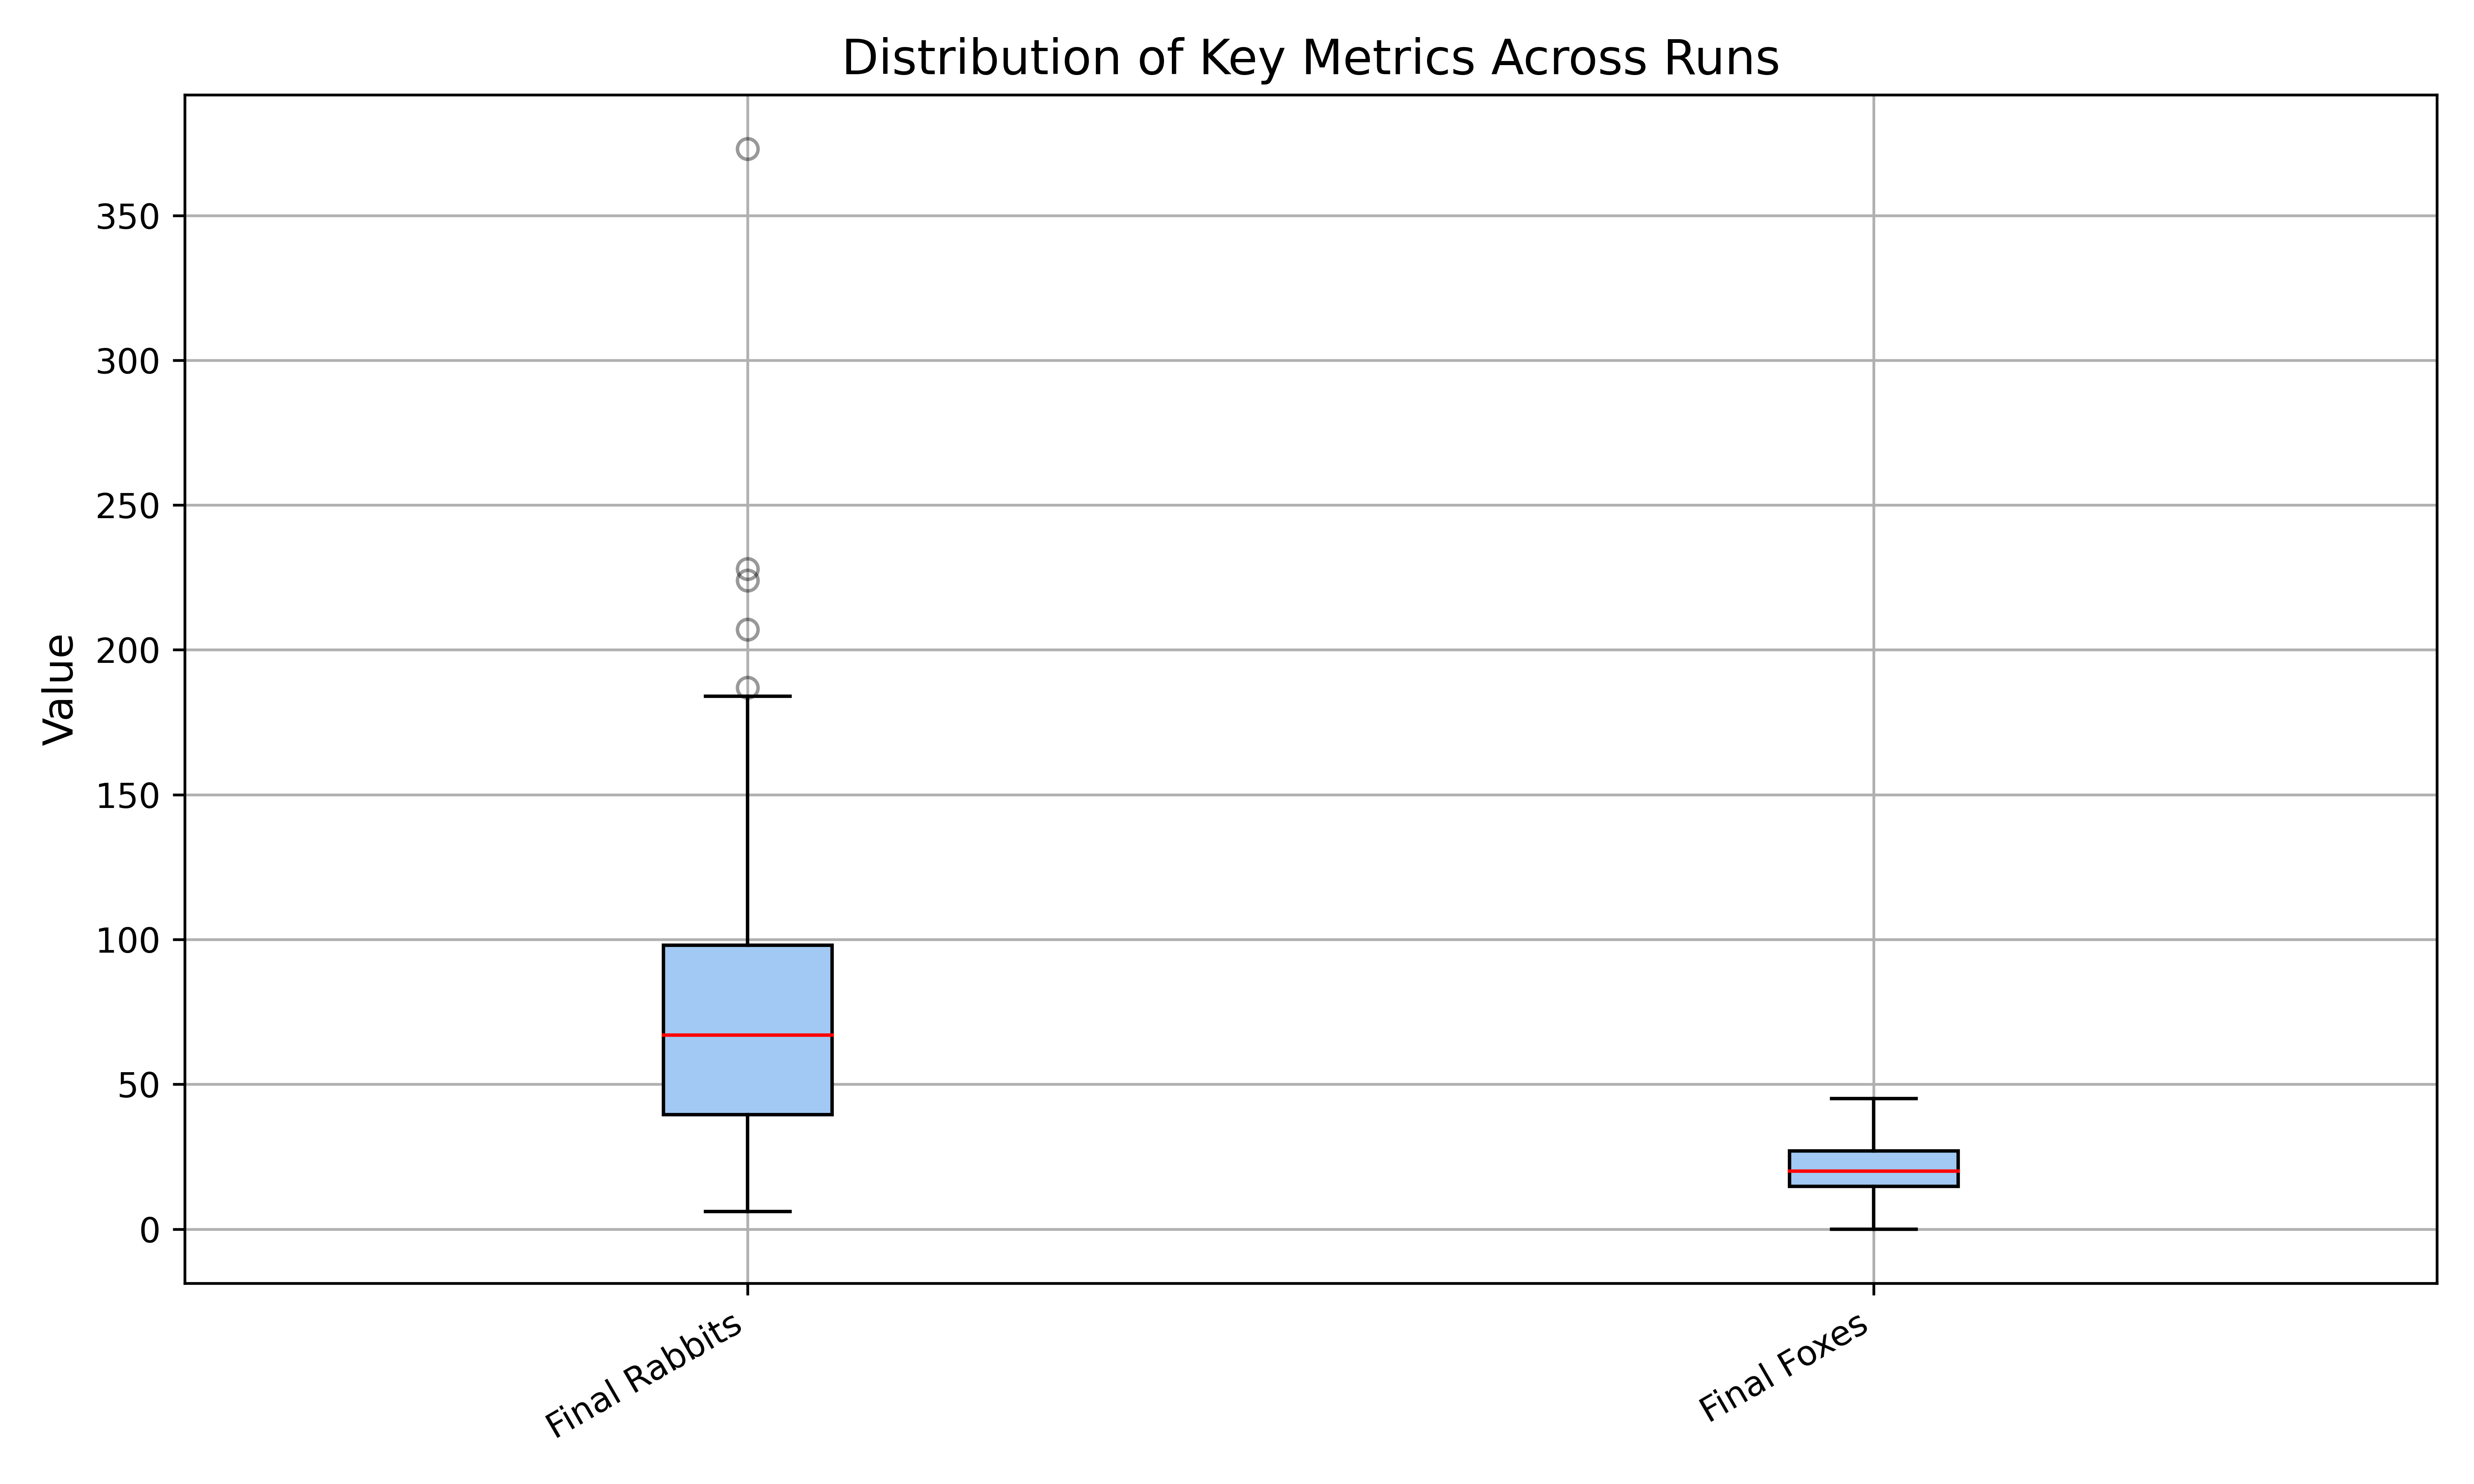
\includegraphics[width=0.9\linewidth]{images/boxplot_metrics_100_sim.png}
  \caption{
    Descriptive statistics of key ecological variables recorded across 100 independent simulation runs of the Agent-Based Model (ABM), with each run spanning up to 1000 iterations. For more information see Table ~\ref{tab:simulation_stats_2.1}.
}
  \label{fig:boxplot_metrics_100_sim}
\end{figure}


\section{Tables}
\listoftables
\begin{table}[h]
\centering
\resizebox{\linewidth}{!}{%
\begin{tabular}{|l|l|p{5cm}|p{5cm}|}
\hline
\textbf{Method} & \textbf{Global Error} & \textbf{Pros} & \textbf{Cons} \\ \hline
Explicit Euler & $O(\Delta t)$ & Simple; low computational cost per step; easy to implement & Poor stability for larger $\Delta t$ in chaotic regimes; error accumulates linearly \\ \hline
RK4 & $O(\Delta t^4)$ & Higher accuracy and stability; better error control over fixed step sizes & More computationally expensive per step; increased complexity compared to Euler \\ \hline
Adaptive Methods (e.g., RK45) & Varies with adaptive step-size & Dynamically adjusts $\Delta t$ based on error; accurate and efficient in varying dynamics & More complex; computational overhead for step adjustment \\ \hline
\end{tabular}%
}
\caption{Comparison of Integration Methods}
\label{tab:integration_methods}
\end{table}



\begin{table}[h!]
    \centering
    \label{tab:diff_two_models_predator_prey}
    \begin{tabular}{|l|p{4.5cm}|p{4.5cm}|}
    \hline
    \textbf{Feature} & \textbf{Agent-Based Modeling (ABM)} & \textbf{Equation-Based Modeling (EBM)} \\
    \hline
    Modeling Units & Represents individual agents, such as each rabbit or fox, capturing their unique behaviors and interactions. & Models populations as continuous variables, focusing on aggregate properties rather than individual entities. \\
    \hline
    Stochasticity & Incorporates a high degree of randomness in agents' movements, births, deaths and so on. & Typically deterministic. \\
    \hline
    Spatiality & Explicitly models space, allowing agents to move and interact within an environment (in our case, a 2D environment). & Generally lacks spatial modeling. \\
    \hline
    Emergence & Enables emergent patterns from simple interaction rules among agents. & Patterns are outcomes of governing equations; less emphasis on emergence. \\
    \hline
    Complex Interactions & Models diverse and complex behaviors at the individual level. & Simplifies interactions by averaging behaviors across the population. \\
    \hline
    Realism & More biologically realistic, but computationally expensive. & Abstract, analytically tractable, and computationally less expensive, but may lack individual-level detail. \\
    \hline
    \end{tabular}
    \caption{Comparison of Agent-Based Modeling (ABM) and Equation-Based Modeling (EBM)}
\end{table}



\section{References}
\bibliographystyle{acm} 
\bibliography{references} 
% \printbibliography
\end{document}
